\documentclass[a4paper]{article}
\usepackage[a4paper,includeheadfoot,margin=2.54cm]{geometry}
\usepackage{listings}
\lstset{language=C++} 
\usepackage{tikz}
\usepackage{pgfplots, pgfplotstable}
\usepackage{graphicx}
\usepackage{amsmath}

\newcommand{\addcustomplot}[4]{	
	{
		%\pgfplotstablegetcolsof{#}
		\addplot[scatter, color=#2,
		scatter/@pre marker code/.style={/tikz/mark size=2.0pt},
		scatter/@post marker code/.style={},
		line width = 1.5pt
		]
		table[x index=0,y index=#3, col sep=comma] {#1};
		\addlegendentryexpanded{#4}
	}
}

\newcommand{\addcustomybarplot}[4]
{
	\addplot[black,pattern color=#3,fill=#3,pattern=north east lines]  table[x index=0,y index=#2,col sep=comma]{#1};
	\addlegendentryexpanded{#4};
}


\newcommand{\plotfile}[1]{
	\pgfplotstableread{#1}{\table}
	\pgfplotstablegetcolsof{#1}
	\pgfmathtruncatemacro\numberofcols{\pgfplotsretval-1}
	\pgfplotsinvokeforeach{1,...,\numberofcols}{
		\pgfplotstablegetcolumnnamebyindex{##1}\of{\table}\to{\colname}
		\addplot table [y index=##1] {#1}; 
		\addlegendentryexpanded{\colname}
	}
}

\newcommand{\stencilpt}[4][]{\node[circle,draw,inner sep=0.1em,minimum size=0.8cm,font=\tiny,#1] at (#2) (#3) {#4}}


\lstset{
	basicstyle=\ttfamily\footnotesize,
	frame=single,
	breaklines=true,
	postbreak=\raisebox{0ex}[0ex][0ex]{\ensuremath{\color{red}\hookrightarrow\space}}
}


% Define block styles
\tikzstyle{decision} = [diamond, draw, fill=blue!20, 
text width=4.5em, text badly centered, node distance=3cm, inner sep=0pt]
\tikzstyle{block} = [rectangle, draw, fill=blue!20, 
 text centered, rounded corners, minimum height=4em, node distance=3cm]
\tikzstyle{line} = [draw, -latex']
\tikzstyle{cloud} = [draw, ellipse,fill=red!20, node distance=3cm,
minimum height=2em]

\begin{document}
	\pagenumbering{gobble}
	
	%----------------------------------------------------------------------------------------
	%	TITLE PAGE
	%----------------------------------------------------------------------------------------
	\begin{titlepage}
		\newcommand{\HRule}{\rule{\linewidth}{0.5mm}}
		
		\center
		
		%----------------------------------------------------------------------------------------
		%	HEADING SECTIONS
		\textsc{\LARGE Cranfield University}\\[1.5cm]
		\textsc{\Large MSc in Computational and Software Techniques in Engineering 2016/2017}\\[0.5cm]
		\textsc{\large Subject}\\[0.5cm]
		
		%----------------------------------------------------------------------------------------
		%	TITLE SECTION
		\HRule \\[0.4cm]
		{ \huge \bfseries Topic}\\[0.4cm]
		\HRule \\[1.5cm]
		
		%----------------------------------------------------------------------------------------
		%	LOGO SECTION
		
\includegraphics[width=8cm]{img/cranfield-logo}\\[1cm]
		
		%----------------------------------------------------------------------------------------
		%	AUTHOR SECTION
		\vfill
		\begin{minipage}{0.4\textwidth}
			\begin{flushleft} \large
				\emph{Author:}\\
				Mateusz \textsc{Gasior}
			\end{flushleft}
		\end{minipage}
		~
		\begin{minipage}{0.4\textwidth}
			\begin{flushright} \large
				\emph{Supervisor:} \\
				NAME \textsc{SURNAME}
			\end{flushright}
		\end{minipage}\\[2cm]
		
		%----------------------------------------------------------------------------------------
		%	DATE SECTION
		\vfill
		{\large \today}
		\clearpage
	\end{titlepage}

	%----------------------------------------------------------------------------------------
	%	TABLE OF CONTENTS
	%----------------------------------------------------------------------------------------
	\tableofcontents
	\newpage
	
	%----------------------------------------------------------------------------------------
	%	LIST OF FIGURES
	%----------------------------------------------------------------------------------------
	\listoffigures
	
	%----------------------------------------------------------------------------------------
	%	LIST OF TABLES
	%----------------------------------------------------------------------------------------
	\listoftables
	\newpage
	
	% ABSTRACT 
		%----------------------------------------------------------------------------------------
	%	ABSTRACT
	% • Self-explanatory without reference to the paper.
	% • Max 2 paragraphs, NO ABBREVIATIONS HERE.
	% • Concisely indicate the experiment, objectives, importance.
	% • Newly observed facts and the conclusions of the experiment.
	% • Only the most significant results should be given.
	%----------------------------------------------------------------------------------------
	\pagenumbering{arabic}
	\begin{abstract}

	\end{abstract}

	%----------------------------------------------------------------------------------------
	%	INTRODUCTION
	% • Statement of the problem investigated.
	% • Background information.
	% • Concise introduction to theory or concepts used.
	% • Subsections.
	%----------------------------------------------------------------------------------------
	
	%----------------------------------------------------------------------------------------
%	INTRODUCTION
% • Statement of the problem investigated.
% • Background information.
% • Concise introduction to theory or concepts used.
% • Subsections.
%----------------------------------------------------------------------------------------
\section{Introduction}
	The numerical methods are fundamental to solve many problems from a real-world. In case of this assignment all work is focused around advection equation which is a physic formula that describes transport of a substance. This is not only branch of science that uses numerical methods in order to solve problems. It is true that physics, engineering and earth sciences are extremely popular branches of science that use numerical approximations for many practical problems. For example in meteorology and physical oceanography, advection often refers to the horizontal transport of some property of the atmosphere or ocean, such as hear, humidity or salinity, and convection generally refers to vertical transport (vertical advection)\footnote{https://en.wikipedia.org/wiki/Advection}. In case of this assignment we talk about about horizontal transport of wave in time. Apart of the problem there are many numerous schemes designed to ensure the best results. There are many existing powerful and flexible tools, but the user of them should be highly aware of the consequences of using them. A key aspect of using numerical schemes is to balance between good accuracy and stability of the scheme.
	
	Stability of the scheme has a pivotal role in ensuring that the solution is meaningful. It also means that we can trust our results, because there is no way to compare our numerical results - there is no analytical solution. The second crucial element for good calculation is examination of grid convergence. If used schema is not convergent, it cannot be used in a practical way. Every schema distorts our solution by introducing vary effects, such as: dissipation or dispersion. Besides of those effects each of the schemes also introduces truncation error. Apart of all factors related to the schemes, there is also a round-off error related to the precision of a computer which may significantly affect our results.
	
	\subsection{Objective}
		The main objective of the assignment is to implement, examine and discuss about four numerical schemes (implicit and explicit upwind, Lax-Wendroff and Richtmyer multi-step) used to solve simple advection equation which is described as follows:
		
		\begin{equation}
			\frac{\partial f}{\partial t} +  u\frac{\partial f}{\partial x} = 0
		\end{equation}
		
		in a domain $x \in [-50,50]$ with $u = 1.75$ and two initial/boundary conditions:
		
		\begin{itemize}
			\item First set
			{
				\begin{equation}
					\begin{split}
						f(x, 0) = \frac{1}{2} (sign(x) + 1) \\
						f(-50, t) = 0 \\
						f(50, t) = 1
					\end{split}
				\end{equation}
			}
			\item Second set
			{
				\begin{equation}
					\begin{split}
						f(x, 0) = \frac{1}{2} exp(-x^2) \\
						f(-50, t) = 0 \\
						f(50, t) = 0.
					\end{split}
				\end{equation}
			}
		\end{itemize}
		
		The analytical solutions for these initial conditions are given respectively:
		
		\begin{itemize}
			\item First set
			{
				\begin{equation}
					f(x, t) = \frac{1}{2} (sign(x - 1.75t) + 1)
				\end{equation}
			}
			\item Second set
			{
				\begin{equation}
					f(x, t) = \frac{1}{2} exp(-(x - 1.75t)^2).
				\end{equation}
			}
		\end{itemize}
	
		Mentioned before analytical solutions and known are will be used in order to the calculate an error. Further analyses will compare errors of each scheme to determine the best numerical solution between them.

	%----------------------------------------------------------------------------------------
	%	METHODS AND PROCEDURES
	% • The experimental design, methods of gathering data.
    % • Subsections.
	%----------------------------------------------------------------------------------------
	%----------------------------------------------------------------------------------------
%	METHODS AND PROCEDURES
% • The experimental design, methods of gathering data.
% • Subsections.
%----------------------------------------------------------------------------------------
\section{General approach} \label{sec:generalApproach}
	Different approaches have been proposed to describe finite difference method in many books. In case of this report I will base on explanation in chapter 3.5 in Computational Techniques for Fluid Dynamics\cite{bib:fletcher} written by C. A. J. Fletcher. The basis for the finite difference method is the construction of a discrete grid, the replacement of the continuous derivatives in the governing partial equations with equivalent finite difference expressions. Mentioned transformation is presented in Figure \ref{fig:schematicOfFDM}\cite{bib:fletcher}[p. 64--65].
	
	\begin{figure}
		\centering
		\begin{tikzpicture}
			% Place nodes
			\node [block] (setUpGrid) {Set up grid};
			\node [block, right of=setUpGrid, align=center] (initDependentVars) 
			{
				Initialise \\ 
				dependent \\ 
				vairables
			};
			\node [block, right =1cm of initDependentVars, align=center] (construct)
			{
				Construct finite difference \\
				analogue of P.D.E and B.C.s
			};			
			\node [block, below of=construct, align=center] (forEach)
			{
					 For each interior grid point (j, n) \\
					 evaluate algorithm to give $T_j^{n+1}$
			};			
			\node [block, left=1cm of forEach, below of=initDependentVars] (timeStep) 
			{
					$t_{n+1} = t_n + \Delta t$
			};
			\node [block, below of=timeStep, align=center] (adjust) 
			{
					Adjust (if necessary) \\
					boundary values \\
					$T_1^{n+1}$ and $T_j^{n+1}$
			};
			\node [decision, left=1cm of adjust] (final) {Final time reached};
			\node [block, below of=final] (solution) {Solution};
			% Draw edges
			\path [line] (setUpGrid) -- (initDependentVars);
			\path [line] (initDependentVars) -- (construct);
			\path [line] (construct) -- (forEach);
			\path [line] (timeStep) -- (forEach);
			\path [line] (forEach) |- (adjust);
			\path [line] (adjust) -- (final);
			\path [line] (final) |- node[above, midway] {no} (timeStep);
			\path [line] (final) -- node[right] {yes} (solution);
		\end{tikzpicture}
		\caption{Schematic of the finite difference solution process.}
		\label{fig:schematicOfFDM}
	\end{figure}

	General approach mentioned before is a core for algorithm for each of discussed schemes (implicit and explicit upwind, Lax-Wendroff and Richtmyer multi-step). After initialization of the grid and other dependent variables choice is made for finite difference analogue which in our case is particular scheme. Next step in the algorithm is to iterate for given amount of time steps and through all the points that consist for grid. After reaching a final time step or time level actual grid is solution for this time level.
	
	\subsection{Analysis of the schemes} \label{sec:analysis}
		This section is devoted to briefly introduce reader about formulations, stencils and stability conditions, which will be described more precisely in appendix\ref{app:stabilities}. All the formulas are using following dependency \ref{for:cfl}, also known as Courant–Friedrichs–Lewy (CFL) number.
		
		\begin{equation}
			\label{for:cfl}
			C = u \frac{\Delta t}{\Delta x},
		\end{equation} 
		
		where $C$ is the CFL number. In initial parameters of advection function \ref{for:advection} give us $u > 0$ and $\Delta X$ is also greater than $0$ because it refers to amount of points in the grid, which cannot be negative and solution for zero points doesn't make sense. The last important parameter is $\Delta t$ which also should be greater than zero, because it is impossible to go back in time. The conclusion from equation \ref{for:cfl} is that the CFL should always be positive in conditions of considered in this report problem. There is a possibility to change this assumptions but, we will lose the ability to use the following equation $\Delta t = \frac{C\Delta x}{u}$.
		
		For all graphical, geometric arrangement of a nodal group that relate to the point of interest by using a numerical approximation routine in this report used is following notations:
		
		\begin{itemize}
			\item blue nodes are points at time step $n$,
			\item green nodes are points at time step $n+1$,
			\item purple nodes are points at time step $n+const$, where $const$ is a number,
			\item directed lines show how relations between points of different time steps,
			\item undirected lines show relations between points of same time step,
			\item if scheme is multi-step there will be number corresponding to the step above directed line.
		\end{itemize}
		
	\subsection{Explicit upwind scheme} \label{sec:explicitUpwind}
		Formula that gives first-order accurate method for our problem is described in book\cite{bib:hoffman} on pages 191 -- 192 in section 6.5 titled Applications to a Linear Problem, which looks as follows:
		
		\begin{align}
			\label{for:explicitUpwind}
			\begin{split}
				\frac{f_i^{n+1} - f_i^n}{\Delta t} + u\frac{f_i^n - f_{i-1}^n}{\Delta x} = \mathcal{O}(\Delta t, \Delta x) \\
				f_i^{n+1} = f_i^n - C(f_i^n - f_{i-1}^n) + \mathcal{O}(\Delta t^2, \Delta x \Delta t)
			\end{split}
		\end{align}
		
		where $C$ is CFL number introduced earlier \ref{for:cfl}. Geometric arrangement of a nodal group that relate to the points of interest used by this scheme is shown in Figure \ref{fig:explicitUpwind}.
		
		\begin{figure}[!htbp]
			\centering
			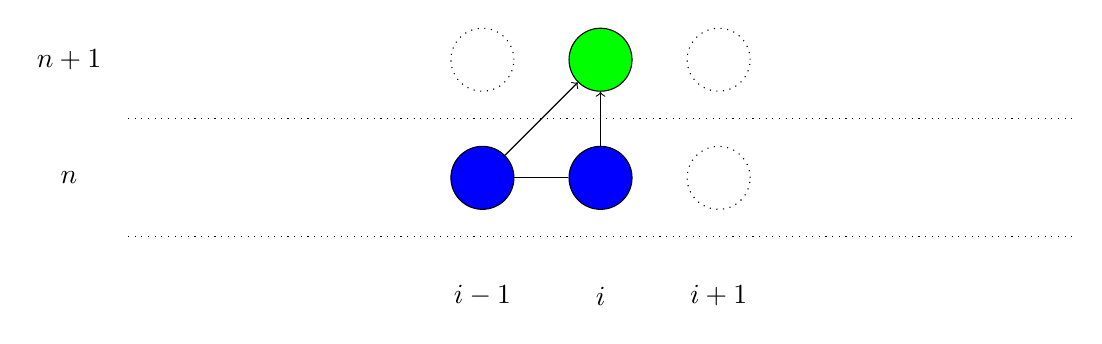
\begin{tikzpicture}[scale=1.5]
			\draw[dotted] (-4,0.5) -- (4,0.5);
			\draw[dotted] (-4,-0.5) -- (4,-0.5);
			\node[black] at (-4.5,1) {$n+1$};
			\node[black] at (-4.5,0) {$n$};
			
			\node[black] at (-1,-1) {$i-1$};
			\node[black] at (0,-1) {$i$};
			\node[black] at (1,-1) {$i+1$};
			
			\stencilpt[fill=blue]{0,0}{ij}{};
			\stencilpt[fill=blue]{-1,0}{i-1j}{};			
			\stencilpt[dotted]{1,0}{i+1j}{};
			
			\stencilpt[fill=green]{0,1}{ij+1}{};
			\stencilpt[dotted]{-1,1}{i-1j+1}{};			
			\stencilpt[dotted]{1,1}{i+1j+1}{};
			\draw (ij) -- (i-1j);
			\draw [->](i-1j) -- (ij+1);
			\draw [->](ij) -- (ij+1);
			
			\end{tikzpicture}
			\caption{Graphical representation of the explicit upwind scheme dependencies.}
			\label{fig:explicitUpwind}
		\end{figure}
		
		Described earlier scheme is first-order accurate both in space and time. Stability analysis in appendix \ref{app:explicitUpwind} shows that this method is conditionally stable for: $C \in (0,1)$.
		
		\subsection{Implicit upwind scheme}
			This formulation uses the FTBS method of finite differencing in the approximation of the PDE in \ref{for:advection}, therefore givin:
			
			\begin{equation}
				\label{for:implicitUpwind_first}
				\frac{f_i^{n+1} - f_i^n}{\Delta t} + u\frac{f_i^{n+1} - f_{i-1}^{n+1}}{\Delta x} = \mathcal{O}(\Delta t, \Delta x)
			\end{equation}
	
			The only known value of $f$ at $i$ is at time $n$. Mentioned dependency drives us to solve following linear equation set of form $Af^{n+1} = f^n$:
			
			\begin{equation}
				\begin{bmatrix}
					1+C & & & \\
					-C & 1+C & & \\ 
					& \ddots & \ddots \\
					& & -C & 1+C \\					
				\end{bmatrix} 
				\times
				\begin{bmatrix}
					f_1^{n+1} \\
					f_2^{n+1} \\
					\vdots	\\
					f_N^{n+1}\\
				\end{bmatrix}
				=
				\begin{bmatrix}
					f_1^{n} + C f_0^{n+1}\\
					f_2^{n} \\
					\vdots	\\
					f_N^{n}\\
				\end{bmatrix},
			\end{equation} 
			
			where $N$ is number of grid points.
			
			The opposite of the previous described explicit upwind method this method is second-order accurate both in time and space. We can observe that we do not have to solve it by using complicated algorithm. Matrix $A$ is bidiagonal diagonally-dominant, so although this schema is implicit we can solve it using forward or backward substitution described using formula \ref{for:implicitSubstitution}. This equation assumes that we know the boundary conditions for next time step - $f_o^{n+1}$ and $f_N^{n+1}$.
			
			\begin{align}
				\label{for:implicitSubstitution}
				\begin{split}
					f_i^{n+1} = \frac{f_i^n + Cf_{i-1}^{n+1}}{1+C}\text{, for $i = 1,2,3,\ldots,N-1$ and $C>0$} \\
					f_{i-1}^{n+1} = \frac{(1+C)f_i^{n+1} - f_i^{n+1}}{C}\text{, for $i = N, N-1, \ldots, 2$ and $C < 0$}
				\end{split}
			\end{align}
			
			Graphical interpretation of this method is shown in Figure \ref{fig:implicitUpwind}.
			
			\begin{figure}[!htbp]
				\centering
				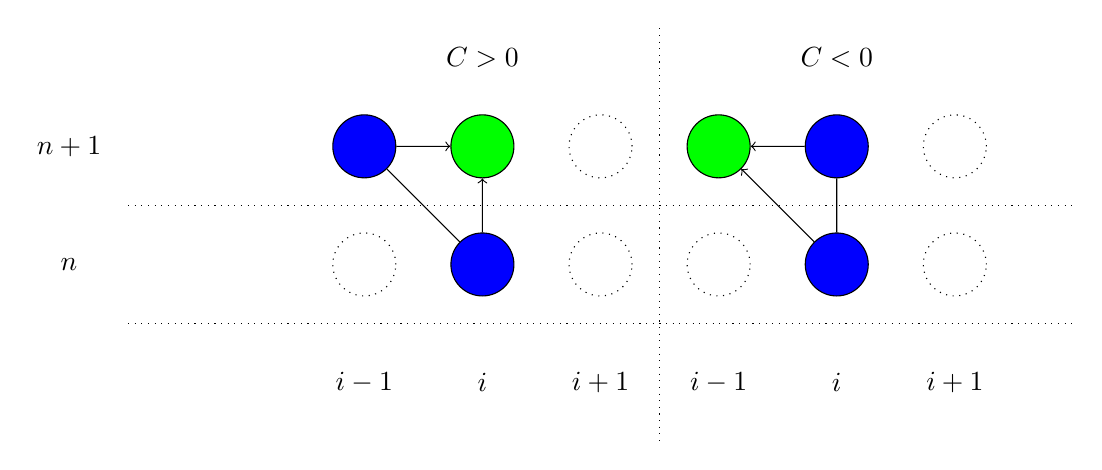
\begin{tikzpicture}[scale=1.5]
					\draw[dotted] (-4,0.5) -- (4,0.5);
					\draw[dotted] (-4,-0.5) -- (4,-0.5);
					\draw[dotted] (0.5, 2) -- (0.5, -1.5);
					
					\node[black] at (-1, 1.75) {$C>0$};
					\node[black] at (2, 1.75) {$C<0$};
					\node[black] at (-4.5,1) {$n+1$};
					\node[black] at (-4.5,0) {$n$};
					
					\node[black] at (-2,-1) {$i-1$};
					\node[black] at (-1,-1) {$i$};
					\node[black] at (0,-1) {$i+1$};
					
					\node[black] at (1,-1) {$i-1$};
					\node[black] at (2,-1) {$i$};
					\node[black] at (3,-1) {$i+1$};
					
					\stencilpt[dotted]{-2,0}{i-2j}{};
					\stencilpt[fill=blue]{-1,0}{i-1j}{};
					\stencilpt[dotted]{0,0}{ij}{};
					\stencilpt[dotted]{1,0}{i+1j}{};	
					\stencilpt[fill=blue]{2,0}{i+2j}{};
					\stencilpt[dotted]{3,0}{i+3j}{};
					
					\stencilpt[fill=blue]{-2,1}{i-2j+1}{};
					\stencilpt[fill=green]{-1,1}{i-1j+1}{};
					\stencilpt[dotted]{0,1}{ij+1}{};
					\stencilpt[fill=green]{1,1}{i+1j+1}{};
					\stencilpt[fill=blue]{2,1}{i+2j+1}{};
					\stencilpt[dotted]{3,1}{i+3j+1}{};
					
					\draw (i-2j+1) -- (i-1j);
					\draw [->](i-2j+1) -- (i-1j+1);
					\draw [->](i-1j) -- (i-1j+1);
					
					\draw (i+2j) -- (i+2j+1);
					\draw [->](i+2j+1) -- (i+1j+1);
					\draw [->](i+2j) -- (i+1j+1);
				\end{tikzpicture}
				\caption{Graphical representation of the implicit upwind scheme dependencies.}
				\label{fig:implicitUpwind}
			\end{figure}
			
			The analysis carried out in appendix \ref{app:implicitUpwind} showed that in general schema is stable for $C \in (-\infty, -1) \cup (0, \infty)$, so in terms of assignment ($C>0$) scheme is unconditionally stable. 
			
			% Should I Mention something about negative CFL?
			
		\subsection{Lax-Wendroff scheme}
			In section 6.2.1.6. in \cite{bib:hoffman}[p. 187] there are considerations about Lax-Wendroff scheme considering problem described by \ref{for:advection}. The finite difference representation of the PDE is derived from Taylor series expansion of the dependent variable as follows: 
			
			\begin{align}
				\begin{split}
					f(x, t + \Delta t) = u(x, t) + u\frac{\partial f}{\partial t}\Delta t + u^2\frac{\partial ^2 f}{\partial t^2}\frac{(\Delta t)^2}{2!} + \mathcal{O}(\Delta t)^3
				\end{split}
			\end{align}		
			
			Considering \ref{for:advection} and calculations provided in \ref{app:lax-wendroff} final formula \ref{for:lax-wenndroffFinal} looks as following, while stencil for Lax-Wendroff scheme is shown in Figure \ref{fig:lax-wendroff}.
			
			\begin{align}
				\label{for:lax-wenndroffFinal}
				\begin{split}
					f_i^{n+1} = f_i^n - \frac{C}{2}(f_{i+1} - f_{i-1}^n) + \frac{C^2}{2}(f_{i+1}^n - 2f_i^n + f_{i-1}^n) + \mathcal{O}(\Delta t^2, \Delta x^2)
				\end{split}
			\end{align}						
			
			\begin{figure}[!htbp]
				\centering
				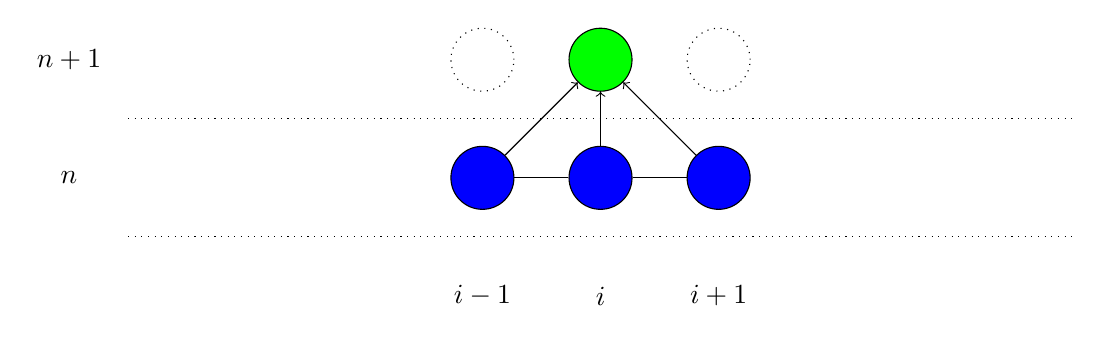
\begin{tikzpicture}[scale=1.5]
				\draw[dotted] (-4,0.5) -- (4,0.5);
				\draw[dotted] (-4,-0.5) -- (4,-0.5);
				\node[black] at (-4.5,1) {$n+1$};
				\node[black] at (-4.5,0) {$n$};
				
				\node[black] at (-1,-1) {$i-1$};
				\node[black] at (0,-1) {$i$};
				\node[black] at (1,-1) {$i+1$};
				
				\stencilpt[fill=blue]{0,0}{ij}{};
				\stencilpt[fill=blue]{-1,0}{i-1j}{};			
				\stencilpt[fill=blue]{1,0}{i+1j}{};
				
				\stencilpt[fill=green]{0,1}{ij+1}{};
				\stencilpt[dotted]{-1,1}{i-1j+1}{};			
				\stencilpt[dotted]{1,1}{i+1j+1}{};
				\draw (ij) -- (i-1j);
				\draw (ij) -- (i+1j);
				\draw [->](i-1j) -- (ij+1);
				\draw [->](ij) -- (ij+1);
				\draw [->](i+1j) -- (ij+1);
				
				\end{tikzpicture}
				\caption{Graphical representation of the Lax-Wendroff scheme dependencies.}
				\label{fig:lax-wendroff}
			\end{figure}
				
			This method is compared to implicit upwind scheme is also second-order accurate both in time and space. Stability analysis in \ref{app:lax-wendroff} shows that this explicit method is stable in symmetric function for $C \in (-1, 0) \cup (0, 1)$. However in case of assignment only positive part will be considered.
			
		\subsection{Richtmyer multi-step scheme}
			In Computation fluid dynamics vol I\cite{bib:hoffman} we can find formulation for each point of a grid on page 190. This method is multi-step because in first step we predict value to the time level $n + \frac{1}{2}$ and using Lax-Fredrich predictor \ref{for:lax-friedrichPredictor}. Next predicted values are used in order to get value for time level $n+1$ by applying it to formula \ref{for:richtmyer-multi-step}.
			
			\begin{equation}
				\label{for:lax-friedrichPredictor}
				f_{i}^{n+\frac{1}{2}} = \frac{1}{2} (f_{i+1}^n - f_{i-1}^n) - \frac{C}{4}(f_{i+1}^n - f_{i-1}^n) + \mathcal{O}(\Delta t^2, \Delta x^2\Delta t)
			\end{equation}
			
			\begin{equation}
				\label{for:richtmyer-multi-step}
				f_i^{n+1} = f_i^n - C(u_{i+1}^{n+\frac{1}{2}} - u_{n-1}^{n+\frac{1}{2}}) + \mathcal{O} (\Delta t^3, \Delta x^2\Delta t)
			\end{equation}
			
			This method is stable for $C \in (-2, 0) \cup (0, 2)$. For the same reason as in Lax-Wendroff scheme in terms of assignment only postivie part will be considered. Also this scheme is second-order accurate in space and time. Stencil for this scheme is shown in Figure \ref{fig:richtmyer-multi-step}.
			
			\begin{figure}[!htbp]
				\centering
				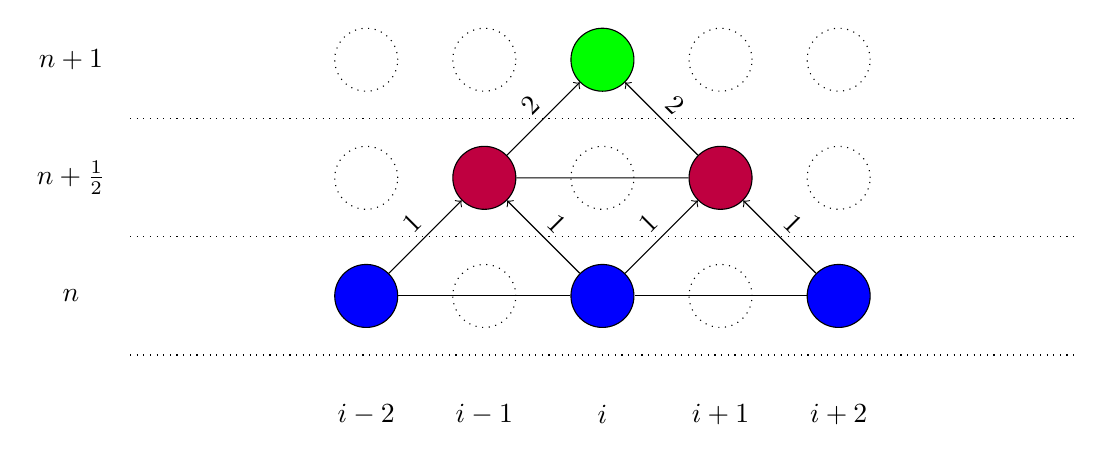
\begin{tikzpicture}[scale=1.5]
				\draw[dotted] (-4,0.5) -- (4,0.5);
				\draw[dotted] (-4,-0.5) -- (4,-0.5);
				\draw[dotted] (-4, 1.5) -- (4, 1.5);
				\node[black] at (-4.5,1) {$n+\frac{1}{2}$};
				\node[black] at (-4.5,0) {$n$};
				\node[black] at (-4.5,2) {$n + 1$};
				
				\node[black] at (-2,-1) {$i-2$};
				\node[black] at (-1,-1) {$i-1$};
				\node[black] at (0,-1) {$i$};
				\node[black] at (1,-1) {$i+1$};
				\node[black] at (2,-1) {$i+2$};
				
				\stencilpt[fill=blue]{-2,0}{i-2j}{};
				\stencilpt[dotted]{-1,0}{i-1j}{};
				\stencilpt[fill=blue]{0,0}{ij}{};
				\stencilpt[dotted]{1,0}{i+1j}{};
				\stencilpt[fill=blue]{2,0}{i+2j}{};
				
				\stencilpt[dotted]{-2,1}{i-2j+1}{};
				\stencilpt[fill=purple]{-1,1}{i-1j+1}{};
				\stencilpt[dotted]{0,1}{ij+1}{};
				\stencilpt[fill=purple]{1,1}{i+1j+1}{};
				\stencilpt[dotted]{2,1}{i+2j+1}{};
				
				\stencilpt[dotted]{-2,2}{i-2j+2}{};
				\stencilpt[dotted]{-1,2}{i-1j+2}{};
				\stencilpt[fill=green]{0,2}{ij+2}{};
				\stencilpt[dotted]{1,2}{i+1j+2}{};
				\stencilpt[dotted]{2,2}{i+2j+2}{};
				
				\draw (i-2j) -- (ij);				
				\draw (ij) -- (i+2j);			
				\draw (i-1j+1) -- (i+1j+1);

				\draw [->] (i-2j) -- node [midway, above, sloped] {1} (i-1j+1);
				\draw [->] (ij) -- node [midway, above, sloped] {1} (i-1j+1);
				\draw [->] (ij) -- node [midway, above, sloped] {1} (i+1j+1);
				\draw [->] (i+2j) -- node [midway, above, sloped] {1} (i+1j+1);
				
				\draw [->] (i-1j+1) -- node [midway, above, sloped] {2} (ij+2);
				\draw [->] (i+1j+1) -- node [midway, above, sloped] {2} (ij+2);
				
				\end{tikzpicture}
				\caption{Graphical representation of the Lax-Wendroff scheme dependencies.}
				\label{fig:richtmyer-multi-step}
			\end{figure}
		
		
	
	%----------------------------------------------------------------------------------------
	%	RESULTS
	% • Heart of the report.
	% • Actual results, implications, errors.
	% • Combine Results and Discussions when the discussion of first result is needed to
	% understand second result.
	% • Tables, figures, Graphs APPROPRIATELY REFERENCED IN THE TEXT.
	% • Figure legends -- below the figure; table legends -- above the table.
	%----------------------------------------------------------------------------------------
	%----------------------------------------------------------------------------------------
%	RESULTS
% • Heart of the report.
% • Actual results, implications, errors.
% • Combine Results and Discussions when the discussion of first result is needed to
% understand second result.
% • Tables, figures, Graphs APPROPRIATELY REFERENCED IN THE TEXT.
% • Figure legends -- below the figure; table legends -- above the table.
%----------------------------------------------------------------------------------------
\chapter{Results} \label{sec:results}
	Each of the schemes works differently, although all of them aspire to give the best numerical solution. In order to compare them for each of mentioned further questions there will be some preset values for discretization parameters.
	This section gives answer for following queries:
	
	\begin{itemize}
		\item How do the numerical solutions vary with the Courant number?
		\item How does the numerical solution change in time?
		\item Examination of grid convergence of numerical solutions at $t=5$.
		\item Explanation of the numerical solutions in terms of the expected properties of the schemes involved.
	\end{itemize}

	\subsection{Impact of the Courant-Friedrichs-Lewy number} \label{sec:impactCFL}
	For all the conducted experiments in this section grid size is equal to $100$. Each of the scheme are described in individual subsection. Therefore quantitative summary of all results is in table \ref{tab:impactCFL}.
	
	\subsection{Explicit upwind}
	\begin{figure}
		\centering	
		\begin{tikzpicture}
		
		\pgfplotsset{width=\textwidth}
		\begin{axis}[
		xlabel = {$x$},
		ylabel = {$y$},
		%ymin = -1, ymax = 1,
		xmin = 0, xmax = 30,
		minor y tick num = 1,
		ymajorgrids=true,
		xmajorgrids=true,
		grid style=dashed,
		legend pos=north west
		]
		
		\addcustomplot{../Code/results/impactExplicit/explicit-upwind-100-sign.conf-chart.csv}{red}{4}{Analytical}
		\addcustomplot{../Code/results/impactExplicit/explicit-upwind-100-sign.conf-chart.csv}{green}{3}{$CFL=0.9625$}
		\addcustomplot{../Code/results/impactExplicit/explicit-upwind-100-sign-CFL-0.8.conf-chart.csv}{purple}{3}{$CFL=0.8$}
		\addcustomplot{../Code/results/impactExplicit/explicit-upwind-100-sign-CFL-0.4.conf-chart.csv}{blue}{3}{$CFL=0.2$}
		\end{axis}
		\end{tikzpicture}
		\caption{Explicit upwind scheme solutions for the initial set \ref{for:firstSet} and various CFL numbers.}
	\end{figure}

	\begin{figure}
	\centering	
	\begin{tikzpicture}
	
	\pgfplotsset{width=\textwidth}
	\begin{axis}[
	xlabel = {$x$},
	ylabel = {$y$},
	%ymin = -1, ymax = 1,
	xmin = 0, xmax = 30,
	minor y tick num = 1,
	ymajorgrids=true,
	xmajorgrids=true,
	grid style=dashed
	]
	
	\addcustomplot{../Code/results/impactExplicit/explicit-upwind-100-exp.conf-chart.csv}{red}{4}{Analytical}
	\addcustomplot{../Code/results/impactExplicit/explicit-upwind-100-exp.conf-chart.csv}{green}{3}{$CFL=0.9975$}
	\addcustomplot{../Code/results/impactExplicit/explicit-upwind-100-exp-CFL-0.8.conf-chart.csv}{purple}{3}{$CFL=0.8$}
	\addcustomplot{../Code/results/impactExplicit/explicit-upwind-100-exp-CFL-0.4.conf-chart.csv}{blue}{3}{$CFL=0.2$}
	\end{axis}
	\end{tikzpicture}
	\caption{Explicit upwind scheme solutions for the initial set \ref{for:secondSet} and various CFL numbers.}
\end{figure}
	\subsection{Implicit upwind}
	\begin{figure}
		\centering	
		\begin{tikzpicture}[scale=0.7]
		
		\pgfplotsset{width=\textwidth}
		\begin{axis}[
		xlabel = {$x$},
		ylabel = {$y$},
		xmin = 2, xmax = 32,
		minor y tick num = 1,
		ymajorgrids=true,
		xmajorgrids=true,
		grid style=dashed,
		legend pos=north west
		]
		
		\addcustomplot{../Code/results/impactImplicit/implicit-upwind-100-sign.conf-chart.csv}{red}{4}{Analytical}
		\addcustomplot{../Code/results/impactImplicit/implicit-upwind-100-sign.conf-chart.csv}{green}{3}{$CFL=0.0175$}
		\addcustomplot{../Code/results/impactImplicit/implicit-upwind-100-sign-CFL-1.1.conf-chart.csv}{purple}{3}{$CFL=1.1$}		\addcustomplot{../Code/results/impactImplicit/implicit-upwind-100-sign-CFL-0.4.conf-chart.csv}{blue}{3}{$CFL=0.4$}
		\end{axis}
		\end{tikzpicture}
		\caption{Implicit upwind scheme solutions for the initial set \ref{for:firstSet} and various CFL numbers.}
	\end{figure}

	\begin{figure}
	\centering	
	\begin{tikzpicture}[scale=0.7]
	
	\pgfplotsset{width=\textwidth}
	\begin{axis}[
	xlabel = {$x$},
	ylabel = {$y$},
	%ymin = -1, ymax = 1,
	xmin = 2, xmax = 32,
	minor y tick num = 1,
	ymajorgrids=true,
	xmajorgrids=true,
	grid style=dashed
	]
	
	\addcustomplot{../Code/results/impactImplicit/implicit-upwind-100-exp.conf-chart.csv}{red}{4}{Analytical}
	\addcustomplot{../Code/results/impactImplicit/implicit-upwind-100-exp.conf-chart.csv}{green}{3}{$CFL=0.0175$}
	\addcustomplot{../Code/results/impactImplicit/implicit-upwind-100-exp-CFL-1.1.conf-chart.csv}{purple}{3}{$CFL=1.1$}
	\addcustomplot{../Code/results/impactImplicit/implicit-upwind-100-exp-CFL-0.4.conf-chart.csv}{blue}{3}{$CFL=0.4$}
	\end{axis}
	\end{tikzpicture}
	\caption{Implicit upwind scheme solutions for the initial set \ref{for:secondSet} and various CFL numbers.}
\end{figure}
	\subsection{Lax-Wendroff}
	Recalling stability of the Lax-Wendroff scheme in terms of assignment gives us condition $CFL \in (0,1)$. This scheme is second-order accurate, hence dispersion errors are expected to be occur. In Figures \ref{fig:laxwendroffSignCFL} and \ref{fig:laxwendroffExpCFL} results are shown and the summary of the calculated is presented in Figure \ref{fig:laxwendroffCFLNorms}. 
	\begin{figure}[!htbp]
		\centering	
		\begin{tikzpicture}[scale=0.5]	
			\pgfplotsset{width=\textwidth}
			\begin{axis}[
				xlabel = {$x$},
				ylabel = {$y$},
				%ymin = -1, ymax = 1,
				xmin = 2, xmax = 32,
				minor y tick num = 1,
				ymajorgrids=true,
				xmajorgrids=true,
				grid style=dashed,
				legend pos=north west,
				ticklabel style={
					/pgf/number format/fixed,
					/pgf/number format/precision=2
				},
				]
				
				\addcustomplot{../Code/results/impactLax-Wendroff/lax-wendroff-100-sign.conf-chart.csv}{red}{4}{Analytical}
				\addcustomplot{../Code/results/impactLax-Wendroff/lax-wendroff-100-sign.conf-chart.csv}{green}{3}{$CFL=0.98$}
				\addcustomplot{../Code/results/impactLax-Wendroff/lax-wendroff-100-sign-CFL-0.8.conf-chart.csv}{purple}{3}{$CFL=0.8$}
				\addcustomplot{../Code/results/impactLax-Wendroff/lax-wendroff-100-sign-CFL-0.4.conf-chart.csv}{blue}{3}{$CFL=0.4$}
			\end{axis}
		\end{tikzpicture}
		\caption{Lax-Wendroff scheme solutions for the initial set (\ref{for:firstSet}) and various CFL numbers.}
		\label{fig:laxwendroffSignCFL}
	\end{figure}
	
	Based on errors presented in Figure \ref{fig:laxwendroffCFLNorms} the best results are obtained with biggest CFL numbers, $0.98$ and $0.9975$, respectively for initial sets (\ref{for:firstSet}) and (\ref{for:secondSet}). The CFL numbers for which the results are the best are close to the one, for which the error should be the smallest, because the solution with this parameter is exact. One of the properties of this scheme is fluctuation and oscillatory behavior of the solution for the relatively small CFL numbers. For $CFL=0.4$ mentioned behavior can be easily and clearly noticed. The maximum amplitude of such oscillatory behavior is increasing during the decrease of the CFL number. The increase of the CFL number anomaly is starts to disappear and for CFL close to 1 it is barely visible. 
	
	\begin{figure}[!hbtp]
		\centering	
		\begin{tikzpicture}[scale=0.5]
		
			\pgfplotsset{width=\textwidth}
			\begin{axis}[
				xlabel = {$x$},
				ylabel = {$y$},
				%ymin = -1, ymax = 1,
				xmin = 2, xmax = 32,
				minor y tick num = 1,
				ymajorgrids=true,
				xmajorgrids=true,
				grid style=dashed,
				ticklabel style={
				/pgf/number format/fixed,
				/pgf/number format/precision=2
				},
				]
				
				\addcustomplot{../Code/results/impactLax-Wendroff/lax-wendroff-100-exp.conf-chart.csv}{red}{4}{Analytical}
				\addcustomplot{../Code/results/impactLax-Wendroff/lax-wendroff-100-exp.conf-chart.csv}{green}{3}{$CFL=0.9975$}
				\addcustomplot{../Code/results/impactLax-Wendroff/lax-wendroff-100-exp-CFL-0.8.conf-chart.csv}{purple}{3}{$CFL=0.8$}
				\addcustomplot{../Code/results/impactLax-Wendroff/lax-wendroff-100-exp-CFL-0.4.conf-chart.csv}{blue}{3}{$CFL=0.4$}
			\end{axis}
		\end{tikzpicture}
		\caption{Lax-Wendroff scheme solutions for the initial set (\ref{for:secondSet}) and various CFL numbers.}
		\label{fig:laxwendroffExpCFL}
	\end{figure}
	
	For both Figure \ref{fig:laxwendroffSignCFL} and \ref{fig:laxwendroffExpCFL} numerical solutions are slightly shifted in phase comparing to the analytical solutions. This behavior can be seen especially for small CFL numbers.
	
	\begin{figure}[!htbp]
		\begin{subfigure}[b]{0.5\textwidth}
			\begin{tikzpicture}
			%\pgfplotsset{width=\textwidth}
				\begin{axis}[
					ybar,
					%symbolic x coords={5,10,15,20},
					xticklabels={$t=5$,$t=10$},
					xtick=data,
					enlarge x limits={abs=2cm},
					ymajorgrids=true,
					xmajorgrids=true,
					grid style=dashed,
					%legend pos=north west
					legend style={at={(0.5,-0.1)},anchor=north,legend cell align=left}
					%nodes near coords,
					%every node near coord/.append style={rotate=90, anchor=west},
					]
					\addcustomybarplot{../Code/results/impactLax-Wendroff/lax-wendroff-100-exp.conf-norms.csv}{2}{green}{$CFL=0.98$};
					\addcustomybarplot{../Code/results/impactLax-Wendroff/lax-wendroff-100-exp-CFL-0.8.conf-norms.csv}{2}{blue}{$CFL=0.8$};
					\addcustomybarplot{../Code/results/impactLax-Wendroff/lax-wendroff-100-exp-CFL-0.4.conf-norms.csv}{2}{purple}{$CFL=0.4$};
				
				\end{axis}
			\end{tikzpicture}
			\caption{Initial set (\ref{for:secondSet}).}
		\end{subfigure}
		\begin{subfigure}[b]{0.5\textwidth}
			\begin{tikzpicture}
				\begin{axis}[
					ybar,
					%symbolic x coords={5,10,15,20},
					xticklabels={$t=5$,$t=10$},
					xtick=data,
					enlarge x limits={abs=2cm},
					ymajorgrids=true,
					xmajorgrids=true,
					grid style=dashed,
					%legend pos=north west
					legend style={at={(0.5,-0.1)},anchor=north,legend cell align=left},
					%nodes near coords,
					%every node near coord/.append style={rotate=90, anchor=west},
					]
					\addcustomybarplot{../Code/results/impactLax-Wendroff/lax-wendroff-100-sign.conf-norms.csv}{2}{green}{$CFL=0.9975$};
					\addcustomybarplot{../Code/results/impactLax-Wendroff/lax-wendroff-100-sign-CFL-0.8.conf-norms.csv}{2}{blue}{$CFL=0.8$};
					\addcustomybarplot{../Code/results/impactLax-Wendroff/lax-wendroff-100-sign-CFL-0.4.conf-norms.csv}{2}{purple}{$CFL=0.4$};
				
				\end{axis}
			\end{tikzpicture}
			\caption{Initial set (\ref{for:firstSet}).}
		\end{subfigure}
		\caption{Distribution of the error (norm 2) among different CFL numbers for Lax-Wendroff scheme.}
		\label{fig:laxwendroffCFLNorms}
	\end{figure}

	Distribution of the error presented in Figure \ref{fig:laxwendroffCFLNorms} shows that error rise with decrease of CFL number. Similarly to other schemes error for (\ref{for:firstSet}) is bigger in this case 2 times.
	\subsection{Richtmyer multi-step}
\begin{figure}
	\centering	
	\begin{tikzpicture}
	
	\pgfplotsset{width=\textwidth}
	\begin{axis}[
	xlabel = {$x$},
	ylabel = {$y$},
	%ymin = -1, ymax = 1,
	xmin = 2, xmax = 32,
	minor y tick num = 1,
	ymajorgrids=true,
	xmajorgrids=true,
	grid style=dashed,
	legend pos=north west
	]
	
	\addcustomplot{../Code/results/impactRichtmyer-Multi-Step/richtmyer-ms-100-sign.conf-chart.csv}{red}{4}{Analytical}
	\addcustomplot{../Code/results/impactRichtmyer-Multi-Step/richtmyer-ms-100-sign.conf-chart.csv}{green}{3}{$CFL=1.96$}
	\addcustomplot{../Code/results/impactRichtmyer-Multi-Step/richtmyer-ms-100-sign-CFL-0.8.conf-chart.csv}{purple}{3}{$CFL=0.8$}
	\addcustomplot{../Code/results/impactRichtmyer-Multi-Step/richtmyer-ms-100-sign-CFL-1.9.conf-chart.csv}{blue}{3}{$CFL=1.9$}
	\end{axis}
	\end{tikzpicture}
	\caption{Richtmyer multi-step scheme solutions for the initial set \ref{for:firstSet} and various CFL numbers.}
\end{figure}

\begin{figure}
	\centering	
	\begin{tikzpicture}
	
	\pgfplotsset{width=\textwidth}
	\begin{axis}[
	xlabel = {$x$},
	ylabel = {$y$},
	%ymin = -1, ymax = 1,
	xmin = 2, xmax = 32,
	minor y tick num = 1,
	ymajorgrids=true,
	xmajorgrids=true,
	grid style=dashed
	]
	
	\addcustomplot{../Code/results/impactRichtmyer-Multi-Step/richtmyer-ms-100-exp.conf-chart.csv}{red}{4}{Analytical}
	\addcustomplot{../Code/results/impactRichtmyer-Multi-Step/richtmyer-ms-100-exp.conf-chart.csv}{green}{3}{$CFL=1.995$}
	\addcustomplot{../Code/results/impactRichtmyer-Multi-Step/richtmyer-ms-100-exp-CFL-0.8.conf-chart.csv}{purple}{3}{$CFL=0.8$}
	\addcustomplot{../Code/results/impactRichtmyer-Multi-Step/richtmyer-ms-100-exp-CFL-1.9.conf-chart.csv}{blue}{3}{$CFL=1.9$}
	\end{axis}
	\end{tikzpicture}
	\caption{Richtmyer multi-step scheme solutions for the initial set \ref{for:secondSet} and various CFL numbers.}
\end{figure}
	
	\begin{table}[]
		\centering
		\caption{Summary of norms for different schemes and initial sets.}
		\label{tab:impactCFL}
				\begin{tabular}{|l|l|l|l|l|l|l|}
					\hline
					\multicolumn{7}{|c|}{\textbf{Explicit upwind}} \\ \hline
					& \multicolumn{3}{|c|}{\textit{\textbf{Sign}}} & \multicolumn{3}{|c|}{\textit{\textbf{Exp}}} \\ \hline
					\multicolumn{1}{|c|}{{\ul \textbf{CFL}}} & \multicolumn{1}{|c|}{{\ul \textbf{Norm }$\infty$}} & \multicolumn{1}{c}{{\ul \textbf{Norm 1}}} & \multicolumn{1}{|c|}{{\ul \textbf{Norm 2}}} & \multicolumn{1}{|c|}{{\ul \textbf{Norm }$\infty$}} & \multicolumn{1}{|c|}{{\ul \textbf{Norm 1}}} & \multicolumn{1}{|c|}{{\ul \textbf{Norm 2}}} \\ \hline \hline
					0.9625 & 0.33721 & 0.00696242 & 0.426226 & 0.0130758 & 0.000327298 & 0.0171315 \\ \hline
					0.8 & 0.437126 & 0.015267 & 0.665857 & 0.250344 & 0.00878393 & 0.358201 \\ \hline
					0.4 & 0.447773 & 0.0260841 & 0.871208 & 0.321412 & 0.0113148 & 0.439042 \\ \hline \hline
					
					\multicolumn{7}{|c|}{\textbf{Implicit upwind}} \\ \hline
					& \multicolumn{3}{|c|}{\textit{\textbf{Sign}}} & \multicolumn{3}{|c|}{\textit{\textbf{Exp}}} \\ \hline
					\multicolumn{1}{|c|}{{\ul \textbf{CFL}}} & \multicolumn{1}{|c|}{{\ul \textbf{Norm }$\infty$}} & \multicolumn{1}{|c|}{{\ul \textbf{Norm 1}}} & \multicolumn{1}{|c|}{{\ul \textbf{Norm 2}}} & \multicolumn{1}{|c|}{{\ul \textbf{Norm }$\infty$}} & \multicolumn{1}{|c|}{{\ul \textbf{Norm 1}}} & \multicolumn{1}{||c|}{{\ul \textbf{Norm 2}}} \\ \hline \hline
					1.1 & 0.495317 & 0.0482448 & 1.18971 & 0.369729 & 0.013552 & 0.49565 \\ \hline
					0.4 & 0.475642 & 0.0395579 & 1.07517 & 0.357042 & 0.0128148 & 0.480709 \\ \hline
					0.0175 & 0.467376 & 0.0337562 & 0.992783 & 0.315467 & 0.0123051 & 0.465734 \\ \hline \hline
					
					\multicolumn{7}{|c|}{\textbf{Lax-Wendroff}} \\ \hline
					& \multicolumn{3}{|c|}{\textit{\textbf{Sign}}} & \multicolumn{3}{|c|}{\textit{\textbf{Exp}}} \\ \hline
					\multicolumn{1}{|c|}{{\ul \textbf{CFL}}} & \multicolumn{1}{|c|}{{\ul \textbf{Norm }$\infty$}} & \multicolumn{1}{|c|}{{\ul \textbf{Norm 1}}} & \multicolumn{1}{|c|}{{\ul \textbf{Norm 2}}} & \multicolumn{1}{|c|}{{\ul \textbf{Norm }$\infty$}} & \multicolumn{1}{|c|}{{\ul \textbf{Norm 1}}} & \multicolumn{1}{|c|}{{\ul \textbf{Norm 2}}} \\ \hline \hline
					0.98 & 0.29005 & 0.00557029 & 0.358408 & 0.0163059 & 0.000399571 & 0.0204625 \\ \hline
					0.8 & 0.427679 & 0.0127055 & 0.564268 & 0.220429 & 0.0081959 & 0.332251 \\ \hline
					0.4 & 0.516192 & 0.020258 & 0.728304 & 0.277539 & 0.0134861 & 0.445979 \\ \hline \hline
											
					\multicolumn{7}{|c|}{\textbf{Richtmyer multi-step}} \\ \hline
					& \multicolumn{3}{|c|}{\textit{\textbf{Sign}}} & \multicolumn{3}{|c|}{\textit{\textbf{Exp}}} \\ \hline
					\multicolumn{1}{|c|}{{\ul \textbf{CFL}}} & \multicolumn{1}{|c|}{{\ul \textbf{Norm }$\infty$}} & \multicolumn{1}{|c|}{{\ul \textbf{Norm 1}}} & \multicolumn{1}{|c|}{{\ul \textbf{Norm 2}}} & \multicolumn{1}{|c|}{{\ul \textbf{Norm }$\infty$}} & \multicolumn{1}{|c|}{{\ul \textbf{Norm 1}}} & \multicolumn{1}{|c|}{{\ul \textbf{Norm 2}}} \\ \hline \hline
					1.995 & 0.380821 & 0.00817055 & 0.46317 & 0.0196272 & 0.000742215 & 0.0317352 \\ \hline
					1.9 & 0.464815 & 0.0118803 & 0.602831 & 0.324497 & 0.00751081 & 0.36502 \\ \hline
					0.8 & 0.570305 & 0.0322748 & 0.928004 & 0.307553 & 0.0163754 & 0.493115 \\ \hline \hline
				\end{tabular}
			\end{table}
	
	\section{Changes in numerical solutions in time}
	This section discuss how numerical solutions accuracy changes in time. For each of the schemes grid size is equal to $400$ in order to decrease quantization errors. In Figure \ref{fig:normsInTime} are presented norms calculated for all schemes and initialization functions.
\begin{figure}[!htbp]
	\begin{subfigure}[b]{0.5\textwidth}
		\begin{tikzpicture}
			\begin{axis}[
				ybar,
				%symbolic x coords={5,10,15,20},
				xticklabels={$t=5$,$t=10$,$t=15$,$t=20$},
				xtick=data,
			%	enlarge x limits={abs=2cm},
				ymajorgrids=true,
				xmajorgrids=true,
				grid style=dashed,
				legend pos=north west
				%legend style={at={(0.5,-0.1)},anchor=north,legend cell align=left},
				%nodes near coords,
				%every node near coord/.append style={rotate=90, anchor=west},
				]
				\addcustomybarplot{../Code/results/changeInTime/explicit-upwind-400-exp.conf-norms.csv}{2}{red}{Exponent};
				\addcustomybarplot{../Code/results/changeInTime/explicit-upwind-400-sign.conf-norms.csv}{2}{green}{Signum};						
			\end{axis}
		\end{tikzpicture}
		\caption{Explicit upwind scheme, $CFL=0.98$}
	\end{subfigure}
	\begin{subfigure}[b]{0.5\textwidth}
		\begin{tikzpicture}
			\begin{axis}[
				ybar,
				%symbolic x coords={5,10,15,20},
				xticklabels={$t=5$,$t=10$,$t=15$,$t=20$},
				xtick=data,
			%	enlarge x limits={abs=2cm},
				ymajorgrids=true,
				xmajorgrids=true,
				grid style=dashed,
				legend pos=north west
				%legend style={at={(0.5,-0.1)},anchor=north,legend cell align=left},
				%nodes near coords,
				%every node near coord/.append style={rotate=90, anchor=west},
				]
				\addcustomybarplot{../Code/results/changeInTime/implicit-upwind-400-exp.conf-norms.csv}{2}{blue}{Exponent};
				\addcustomybarplot{../Code/results/changeInTime/implicit-upwind-400-sign.conf-norms.csv}{2}{black}{Signum};						
			\end{axis}
  		\end{tikzpicture}
		\caption{Implicit upwind scheme, $CFL=0.07$}
	\end{subfigure}
	\begin{subfigure}[b]{0.5\textwidth}
		\begin{tikzpicture}
			\begin{axis}[
				ybar,
				%symbolic x coords={5,10,15,20},
				xticklabels={$t=5$,$t=10$,$t=15$,$t=20$},
				xtick=data,
			%	enlarge x limits={abs=2cm},
				ymajorgrids=true,
				xmajorgrids=true,
				grid style=dashed,
				legend pos=north west
				%legend style={at={(0.5,-0.1)},anchor=north,legend cell align=left},
				%nodes near coords,
				%every node near coord/.append style={rotate=90, anchor=west},
				]
				\addcustomybarplot{../Code/results/changeInTime/lax-wendroff-400-exp.conf-norms.csv}{2}{yellow}{Exponent};
				\addcustomybarplot{../Code/results/changeInTime/lax-wendroff-400-sign.conf-norms.csv}{2}{brown}{Signum};						
			\end{axis}
		\end{tikzpicture}
		\caption{Lax-Wendroff scheme, $CFL=0.98$}
	\end{subfigure}
	\begin{subfigure}[b]{0.5\textwidth}
		\begin{tikzpicture}
			\begin{axis}[
				ybar,
				%symbolic x coords={5,10,15,20},
				xticklabels={$t=5$,$t=10$,$t=15$,$t=20$},
				xtick=data,
			%	enlarge x limits={abs=2cm},
				ymajorgrids=true,
				xmajorgrids=true,
				grid style=dashed,
				legend pos=north west
				%legend style={at={(0.5,-0.1)},anchor=north,legend cell align=left},
				%nodes near coords,
				%every node near coord/.append style={rotate=90, anchor=west},
				]
				\addcustomybarplot{../Code/results/changeInTime/richtmyer-ms-400-exp.conf-norms.csv}{2}{purple}{Exponent};
				\addcustomybarplot{../Code/results/changeInTime/richtmyer-ms-400-sign.conf-norms.csv}{2}{orange}{Signum};
										
			\end{axis}
		\end{tikzpicture}
		\caption{Richtmyer multi-step scheme, $CFL=1.96$}
	\end{subfigure}
	\caption{Comparison of distribution of error (norm 1) for different schemes among different time steps, for given CFL numbers.}
	\label{fig:normsInTime}
\end{figure}
 It is easy to observe that for all schemes and initialization functions error grows in time. The errors of each scheme are accumulating with time. Errors	differ from each other for different initialization functions. For initialization set (\ref{for:firstSet}) calculated norms are higher at least two times for each scheme, comparing to initialization set (\ref{for:secondSet}). The graphical representation for each of schemes and initialization sets in presented in appendix \ref{app:changeInTime}.
 \clearpage		
	
	\subsection{Grid convergence}
	A finite difference scheme is said to be convergent if the solution of the discretized equations tends to the exact solution of the differential equation as the grid spacing tends to zero. Mentioned earlier definition is used in \cite{bib:ferzinger}[p. 32] and \cite{bib:hoffman}[p. 23]. Further discussion about this topic is in section 5.7 (Convergence Criteria and Iteration Errors) in \cite{bib:ferzinger}[from p. 124]. Adaptation of this criteria can be used in order to make comparison between schemes. Summarizing the methods involves comparison of two successively refined grids. The higher ratio we get the better solution we have in terms of calculated error (norm).
	\begin{figure}
		\centering
		\begin{tikzpicture}[scale=0.7]	 	
			\pgfplotsset{width=\textwidth}
			\begin{axis}[
				xlabel = {$x$},
				ylabel = {$y$},
				%ymin = -1, ymax = 1,
				xmin = 5, xmax = 13,
				minor y tick num = 1,
				ymajorgrids=true,
				xmajorgrids=true,
				grid style=dashed,
				legend pos=north east
				]
		
			\addcustomplot{../Code/results/gridConvergence/explicit-upwind-400-exp.conf-chart.csv}{red}{2}{Analytical}			 	
			\addcustomplot{../Code/results/gridConvergence/explicit-upwind-100-exp.conf-chart.csv}{blue}{1}{$\Delta x=1$}			 	
			\addcustomplot{../Code/results/gridConvergence/explicit-upwind-200-exp.conf-chart.csv}{purple}{1}{$\Delta x=0.5$}	
			\addcustomplot{../Code/results/gridConvergence/explicit-upwind-400-exp.conf-chart.csv}{black}{1}{$\Delta x=0.25$}
		\end{axis}
		\end{tikzpicture}
		\caption{Explicit upwind scheme solutions for the initial set \ref{for:secondSet} for different, time step 5, $CFL=1.9$.}
	\end{figure}

	\begin{figure}
		\centering
		\begin{tikzpicture}[scale=0.7]	 	
			\pgfplotsset{width=\textwidth}
			\begin{axis}[
				xlabel = {$x$},
				ylabel = {$y$},
				%ymin = -1, ymax = 1,
				xmin = 2, xmax = 16,
				minor y tick num = 1,
				ymajorgrids=true,
				xmajorgrids=true,
				grid style=dashed,
				legend pos=north east
				]
	
				\addcustomplot{../Code/results/gridConvergence/implicit-upwind-400-exp.conf-chart.csv}{red}{2}{Analytical}			 	
				\addcustomplot{../Code/results/gridConvergence/implicit-upwind-100-exp.conf-chart.csv}{blue}{1}{$\Delta x=1$}			 	
				\addcustomplot{../Code/results/gridConvergence/implicit-upwind-200-exp.conf-chart.csv}{purple}{1}{$\Delta x=0.5$}	
				\addcustomplot{../Code/results/gridConvergence/implicit-upwind-400-exp.conf-chart.csv}{black}{1}{$\Delta x=0.25$}
			\end{axis}
		\end{tikzpicture}
		\caption{Implicit upwind scheme solutions for the initial set \ref{for:secondSet} for different grid sizes, time step 5, $CFL=0.4$5.}
	\end{figure}

	\begin{figure}
		\centering
		\begin{tikzpicture}[scale=0.7]	 	
			\pgfplotsset{width=\textwidth}
			\begin{axis}[
				xlabel = {$x$},
				ylabel = {$y$},
				%ymin = -1, ymax = 1,
				xmin = 2, xmax = 16,
				minor y tick num = 1,
				ymajorgrids=true,
				xmajorgrids=true,
				grid style=dashed,
				legend pos=north east
				]
			
				\addcustomplot{../Code/results/gridConvergence/lax-wendroff-400-exp.conf-chart.csv}{red}{2}{Analytical}			 	
				\addcustomplot{../Code/results/gridConvergence/lax-wendroff-100-exp.conf-chart.csv}{blue}{1}{$\Delta x=1$}			 	
				\addcustomplot{../Code/results/gridConvergence/lax-wendroff-200-exp.conf-chart.csv}{purple}{1}{$\Delta x=0.5$}	
				\addcustomplot{../Code/results/gridConvergence/lax-wendroff-400-exp.conf-chart.csv}{black}{1}{$\Delta x=0.25$}
			\end{axis}
		\end{tikzpicture}
		\caption{Lax-Wendroff scheme solutions for the initial set \ref{for:secondSet} for different grid sizes, time step 5, $CFL=0.8$.}
	\end{figure}

	\begin{figure}
		\centering
		\begin{tikzpicture}[scale=0.7]	 	
			\pgfplotsset{width=\textwidth}
			\begin{axis}[
				xlabel = {$x$},
				ylabel = {$y$},
				%ymin = -1, ymax = 1,
				xmin = 2, xmax = 16,
				minor y tick num = 1,
				ymajorgrids=true,
				xmajorgrids=true,
				grid style=dashed,
				legend pos=north east
				]
		
				\addcustomplot{../Code/results/gridConvergence/richtmyer-multi-step-400-exp.conf-chart.csv}{red}{2}{Analytical}			 	
				\addcustomplot{../Code/results/gridConvergence/richtmyer-multi-step-100-exp.conf-chart.csv}{blue}{1}{$\Delta x=1$}			 	
				\addcustomplot{../Code/results/gridConvergence/richtmyer-multi-step-200-exp.conf-chart.csv}{purple}{1}{$\Delta x=0.5$}	
				\addcustomplot{../Code/results/gridConvergence/richtmyer-multi-step-400-exp.conf-chart.csv}{black}{1}{$\Delta x=0.25$}
			\end{axis}
		\end{tikzpicture}
		\caption{Richtmyer multi-step scheme solutions for the initial set \ref{for:secondSet} for different grid sizes, time step 5, $CFL=1.9$.}
	\end{figure}

	\begin{table}[]
		\centering
		\caption[Norm-one errors for different schemes and grid sizes for time level 5.]
		{Norm-one errors for different schemes and grid sizes for time level 5. CFL numbers are 0.8, 0.4, 0.8, 1.9 respectively for explicit, implicit, Lax-Wendroff and Richtmyer multi-step schemes.}
		\label{tab:gridConvergence}
			\begin{tabular}{cl|c|c|c|}
				\cline{3-5}
				\textit{\textbf{}} &  & \multicolumn{3}{c|}{{\ul \textit{\textbf{$\Delta x$}}}} \\ \cline{1-1} \cline{3-5} 
				\multicolumn{1}{|c|}{{\ul \textit{\textbf{Schema}}}} &  & \textit{\textbf{1}} & \textit{\textbf{0.5}} & \textit{\textbf{0.25}} \\ \hline \hline
				\multicolumn{1}{|c|}{\multirow{2}{*}{\textbf{Explicit upwind}}} & Sign & 0.11334 & 0.00763315 & 0.00573018 \\ \cline{2-5} 
				\multicolumn{1}{|l|}{} & Exp & 0.00645338 & 0.00433326 & 0.00297971 \\ \hline \hline
				\multicolumn{1}{|c|}{\multirow{2}{*}{\textbf{Implicit upwind}}} & Sign & 0.0278933 & 0.019779 & 0.0140375 \\ \cline{2-5} 
				\multicolumn{1}{|c|}{} & Exp & 0.0115807 & 0.00975126 & 0.00780818 \\ \hline \hline
				\multicolumn{1}{|c|}{\multirow{2}{*}{\textbf{Lax-Wendroff}}} & Sign & 0.00916075 & 0.0063511 & 0.00458095 \\ \cline{2-5} 
				\multicolumn{1}{|c|}{} & Exp & 0.00560617 & 0.00324702 & 0.0012723 \\ \hline \hline 
				\multicolumn{1}{|c|}{\multirow{2}{*}{\textbf{Richtmyer multi-step}}} & Sign & 0.0091853 & 0.00594017 & 0.00392881 \\ \cline{2-5} 
				\multicolumn{1}{|c|}{} & Exp & 0.0054888 & 0.0028407 & 0.00109077 \\ \hline
			\end{tabular}
		\end{table}
	
	\section{Comparison of schemes}
	In order to completely summarize results of discretization process for advection function comparison is made based on the norm 1. Calculations are made for both initial sets for grid size equal to $400$ and for time level $5$ to describe get the most accurate solution. CFL numbers were chosen based on search criteria, which checked all the possible values for given range of $\Delta t$. Figure \ref{fig:compSign} shows results for (\ref{for:firstSet}), similarly to Figure \ref{fig:compExp}, which describes solutions for initial set (\ref{for:secondSet}).
	\begin{figure}[!htbp]
		\centering
		\begin{tikzpicture}[scale=0.5]	 	
			\pgfplotsset{width=\textwidth}
			\begin{axis}[
				xlabel = {$x$},
				ylabel = {$y$},
				%ymin = -1, ymax = 1,
				xmin = 5, xmax = 13,
				minor y tick num = 1,
				ymajorgrids=true,
				xmajorgrids=true,
				grid style=dashed,
				ticklabel style={
					/pgf/number format/fixed,
					/pgf/number format/precision=2
				},
				legend pos=south east
				]
		
				\addcustomplot{../Code/results/comparision/implicit-upwind-400-sign.conf-chart.csv}{red}{2}{Analytical}			 	
				\addcustomplot{../Code/results/comparision/implicit-upwind-400-signComp.conf-chart.csv}{green}{1}{Implicit upwind $CFL=0.07$}			
				\addcustomplot{../Code/results/comparision/explicit-upwind-400-sign.conf-chart.csv}{blue}{1}{Explicit upwind $CFL=0.98$}			 	
				\addcustomplot{../Code/results/comparision/lax-wendroff-400-sign.conf-chart.csv}{purple}{1}{Lax-Wendroff $CFL=0.98$}	
				\addcustomplot{../Code/results/comparision/richtmyer-multi-step-400-sign.conf-chart.csv}{black}{1}{Richtmyer multi-step $CFL=1.96$}
			\end{axis}
		\end{tikzpicture}
		\caption{Comparison of schemes for initial set (\ref{for:firstSet}), 400 grid size, time level 5, and different CFLs.}
		\label{fig:compSign}
	\end{figure}
	
	\begin{figure}[!htbp]
		\centering
		\begin{tikzpicture}[scale=0.5]	 	
			\pgfplotsset{width=\textwidth}
				\begin{axis}[
				xlabel = {$x$},
				ylabel = {$y$},
				%ymin = -1, ymax = 1,
				xmin = 5, xmax = 14,
				minor y tick num = 1,
				ymajorgrids=true,
				xmajorgrids=true,
				grid style=dashed,
				ticklabel style={
					/pgf/number format/fixed,
					/pgf/number format/precision=2
				},
				legend pos=north east
				]
			
				\addcustomplot{../Code/results/comparision/implicit-upwind-400-exp.conf-chart.csv}{red}{2}{Analytical}			 	
				\addcustomplot{../Code/results/comparision/implicit-upwind-400-expComp.conf-chart.csv}{green}{1}{Implicit upwind $CFL=0.07$}			
				\addcustomplot{../Code/results/comparision/explicit-upwind-400-exp.conf-chart.csv}{blue}{1}{Explicit upwind $CFL=0.98$}			 	
				\addcustomplot{../Code/results/comparision/lax-wendroff-400-exp.conf-chart.csv}{purple}{1}{Lax-Wendroff $CFL=0.98$}	
				\addcustomplot{../Code/results/comparision/richtmyer-multi-step-400-exp.conf-chart.csv}{black}{1}{Richtmyer multi-step $CFL=1.96$}
			\end{axis}
		\end{tikzpicture}
		\caption{Comparison of schemes for initial set (\ref{for:secondSet}), 400 grid size, time level 5, and different CFLs.}
		\label{fig:compExp}
	\end{figure}
	Error distribution in Figure \ref{fig:errorsComparison} shows clearly that Lax-Wendroff scheme for 
	\begin{figure}[!htbp]
		\begin{subfigure}[b]{0.5\textwidth}
			\begin{tikzpicture}
				%\pgfplotsset{width=\textwidth}
				\begin{axis}[
					ybar,
					%symbolic x coords={5,10,15,20},
					xticklabels={$t=5$,$t=10$},
					xtick=data,
					enlarge x limits={abs=2cm},
					ymajorgrids=true,
					xmajorgrids=true,
					grid style=dashed,
					%legend pos=north west
					legend style={at={(0.5,-0.1)},anchor=north,legend cell align=left}
					%nodes near coords,
					%every node near coord/.append style={rotate=90, anchor=west},
					]
					\addcustomybarplot{../Code/results/comparision/implicit-upwind-400-signComp.conf-norms.csv}{2}{yellow}{Implicit upwind};
					\addcustomybarplot{../Code/results/comparision/explicit-upwind-400-sign.conf-norms.csv}{2}{red}{Explicit upwind};
					\addcustomybarplot{../Code/results/comparision/lax-wendroff-400-sign.conf-norms.csv}{2}{blue}{Lax-Wendroff};
					\addcustomybarplot{../Code/results/comparision/richtmyer-multi-step-400-sign.conf-norms.csv}{2}{green}{Richtmyer multi-step};
				
				\end{axis}
			\end{tikzpicture}
			\caption{Initial set (\ref{for:firstSet}).}
		\end{subfigure}
		\begin{subfigure}[b]{0.5\textwidth}
			\begin{tikzpicture}
			\begin{axis}[
			ybar,
			%symbolic x coords={5,10,15,20},
			xticklabels={$t=5$,$t=10$},
			xtick=data,
			enlarge x limits={abs=2cm},
			ymajorgrids=true,
			xmajorgrids=true,
			grid style=dashed,
			%legend pos=north west
			legend style={at={(0.5,-0.1)},anchor=north,legend cell align=left},
			%nodes near coords,
			%every node near coord/.append style={rotate=90, anchor=west},
			]
			\addcustomybarplot{../Code/results/comparision/implicit-upwind-400-expComp.conf-norms.csv}{2}{yellow}{Implicit upwind};
			\addcustomybarplot{../Code/results/comparision/explicit-upwind-400-exp.conf-norms.csv}{2}{red}{Explicit upwind};
			\addcustomybarplot{../Code/results/comparision/lax-wendroff-400-exp.conf-norms.csv}{2}{blue}{Lax-Wendroff};
			\addcustomybarplot{../Code/results/comparision/richtmyer-multi-step-400-exp.conf-norms.csv}{2}{green}{Richtmyer multi-step};
			\end{axis}
			\end{tikzpicture}
			\caption{Initial set (\ref{for:secondSet}).}
		\end{subfigure}
		\caption{Errors (norm 1) for the best acquired solutions for both initial function sets, 400 grid points.}
		\label{fig:errorsComparison}
	\end{figure}
	
		
		
		
	
	%----------------------------------------------------------------------------------------
	%	DISCUSSION
	% • Interpretation
	% • Any patterns/relationships/correlations that were observed that were important.
	%----------------------------------------------------------------------------------------
		%----------------------------------------------------------------------------------------
	%	DISCUSSION
	% • Interpretation
	% • Any patterns/relationships/correlations that were observed that were important.
	%----------------------------------------------------------------------------------------
	\section{Discussion}
	
	%----------------------------------------------------------------------------------------
	%	FUTURE WORK
	% If the results are not definitive, specific future work that may be needed can be
	% (briefly) described.
	%----------------------------------------------------------------------------------------
	
	%----------------------------------------------------------------------------------------
%	FUTURE WORK
% If the results are not definitive, specific future work that may be needed can be
% (briefly) described.
%----------------------------------------------------------------------------------------
\section{Future Work}
	
	%----------------------------------------------------------------------------------------
	%	CONCLUSIONS
	% • What the author thinks the results mean based on the observations.
	% • Should relate directly back to the problem/question stated in the introduction.
	% • DO NOT INTRODUCE SURPRISES HERE
	%----------------------------------------------------------------------------------------
	
	%----------------------------------------------------------------------------------------
%	CONCLUSIONS
% • What the author thinks the results mean based on the observations.
% • Should relate directly back to the problem/question stated in the introduction.
% • DO NOT INTRODUCE SURPRISES HERE
%----------------------------------------------------------------------------------------

\chapter{Conclusion}

	%----------------------------------------------------------------------------------------
	%	ACKNOWLEGEMENTS
	%----------------------------------------------------------------------------------------
	
	\input{acknowledments.tex}
	
	%----------------------------------------------------------------------------------------
	%	ADDITIONAL FEATURES
	%----------------------------------------------------------------------------------------
	%\begin{figure}
	\centering
	\begin{tikzpicture}[scale=0.7]
		\pgfplotsset{width=\textwidth}
		\begin{axis}[
			ybar,
			%symbolic x coords={5,10,15,20},
			xticklabels={$t=5$,$t=10$,$t=15$,$t=20$},
			xtick=data,
			ymajorgrids=true,
			xmajorgrids=true,
			grid style=dashed,
			legend pos=north west
			%nodes near coords,
			%every node near coord/.append style={rotate=90, anchor=west},
			]
			\addcustomybarplot{lax-wendroff-400-exp.conf-norms.csv}{2}{yellow}{Legen1d};
			\addcustomybarplot{explicit-upwind-400-exp.conf-norms.csv}{2}{red}{Lege3nd};
			\addcustomybarplot{lax-wendroff-400-exp.conf-norms.csv}{2}{blue}{Legen2d};
			%\addcustomybarplot{implicit-upwind-200-exp.conf-norms.csv}{2}{green}{Leg4end};
		\end{axis}
	\end{tikzpicture}
	\caption{Super CaPTION}
\end{figure}
	
		
	%----------------------------------------------------------------------------------------
	%	REFERENCES
	%----------------------------------------------------------------------------------------
	\begin{thebibliography}{9}
		
		\bibitem{intro}
		S. Scott Collis,
		\emph{An Introduction to Numerical Analysis for Computational Fluid Mechanics}.
		Sandia National Laboratories,
		April 26, 2005.
		
	\end{thebibliography}

	%----------------------------------------------------------------------------------------
	%	APPENDICES
	% • Pseudocode
	% • Program listing
	% • Information that is too detailed to be placed into the report's text.
	% • Information that does not directly concern the experiment's objectives.
	%----------------------------------------------------------------------------------------
	
	%----------------------------------------------------------------------------------------
%	APPENDICES
% • Pseudocode
% • Program listing
% • Information that is too detailed to be placed into the report's text.
% • Information that does not directly concern the experiment's objectives.
%----------------------------------------------------------------------------------------
\begin{appendix}
	\chapter{Stabilities}\label{app:stabilities}
		%\section{Formulation and stability analysis of explicit upwind scheme}
	Formula that gives first-order accurate method for our problem is described by Klaus A. Hoffman and Steve T. Chiang in \cite{bib:hoffman}[p. 191 - 192] in section 6.5 titled Applications to a Linear Problem, which looks as follows:
		\begin{align}
			\label{app:for:explicitUpwind}
			\begin{split}
				\frac{u_j^{n+1} - u_j^n}{\Delta t} + a\frac{u_j^n - u_{j-1}^n}{\Delta x} = \mathcal{O}(\Delta t, \Delta x)
			\end{split}
		\end{align}
	where $j$ is related to discretized point, $a$ is acceleration of advection function and $n$ is current time step. This scheme uses Forward-Time Backward-Space (FTBS) discretization.
	The only unknown variable in (\ref{app:for:explicitUpwind}) is $f_i^{n+1}$, because it is explicit scheme, for which we can compute solution without solving set of equation. Solution for unknown presents:
	
		\begin{align}
			\label{app:for:explicitUpwindSolution}
			\begin{split}
				u_j^{n+1} = u_j^n - C(u_j^n - u_{j-1}^n) + \mathcal{O}(\Delta t^2, \Delta x \Delta t)
			\end{split}			
		\end{align}
	where $C=\frac{u\Delta t}{\Delta x}$ is Courant-Friedrichs-Lewy (CFL) number.	
	From equation (\ref{app:for:explicitUpwindSolution}) von Neumann Analysis will be carried out. Starting with following equation:
	\begin{equation}
		\label{app:for:explicit}
		u_j^{(n+1)} = u_j^{(n)} - C\Big(u_j^{(n)} - u_{j-1}^{(n)}\Big)
	\end{equation}	
	Key to the von Neumann's analysis is assuming that the solution to the difference equation is of the form:
	\begin{equation}
		\label{app:for:vnkey}
		u_j^{(n)} = \sigma^ne^{ikx_j}
	\end{equation}	
	Recall that $e^{ikx_j} = cos(kx_j) + isin(kx_j)$. Substituting (\ref{app:for:vnkey}) into (\ref{app:for:explicit}) results in:
	
	\begin{align}
		\begin{split}
			\sigma ^{n+1}e^{ikx_j} = \sigma^{n}{e^{ikx_j}} - C(\sigma ^{n}e^{ikx_j} - \sigma ^{n}e^{ikx_{j-1}}) \\
		\end{split}
	\end{align}
	Noting that	
	\begin{align}
		\begin{split}
			x_{j+1} &= x_j + \Delta x \\
			x_{j-1} &= x_j - \Delta x
		\end{split}
	\end{align}	
	and dividing through by $u_j^{(n)} = \sigma^ne^{ikx_j}$ we obtain
	\begin{align}
		\begin{split}
			\sigma &= 1 - C\Big(1 - \frac{e^{ikx_{j-1}}}{e^{ikx_j}}\Big) \\
			\sigma &= 1 - C\Big(1 - \frac{e^{ik (x_j - \Delta x)}}{e^{ikx_j}}\Big) \\
			\sigma &= 1 - C\Big(1 - e^{-ik\Delta x}\Big) \\
		\end{split}
	\end{align}
	The method is stable if the amplification factor is less or equal to 1. The magnitude of the amplification factor is:
	\begin{align}
		\begin{split}
			\label{app:for:sigmaExplicit}
			|\sigma|^2 &= \Bigg( 1 - C\Big(1 - e^{-ik\Delta x}\Big)\Bigg)^2 \\
			&= \Bigg( 1 - C\Big(1 -\cos(k\Delta x) + i\sin(k\Delta x)\Big)\Bigg)^2 \\
			&= \Bigg(1 - C\Big(1 -\cos(k\Delta x)\Big) - iC\sin(k\Delta x)\Bigg)^2 \\	
			&= 1 - 2C\Big(1 - \cos(k\Delta x)\Big) + C^2\Big(1 -\cos(k\Delta x)\Big)^2 + C^2\sin^2(k\Delta x)
		\end{split}
	\end{align} 	
	but	
	\begin{align}
		\begin{split}
			\label{app:for:dependencyExplicit}
			C^2\Big(1 -\cos(k\Delta x)\Big)^2 + C^2\sin^2(k\Delta x) &=C^2\Bigg(1 - 2\cos(k\Delta x) + \cos^2(k\Delta x)\Bigg) + C^2\sin^2(k\Delta x) \\
			&= C^2(1-2\cos(k\Delta x)) + C^2 \\
			&= 2C^2(1-\cos(k\Delta x)))
		\end{split}
	\end{align} 	
	Using dependency (\ref{app:for:dependencyExplicit}) for (\ref{app:for:sigmaExplicit}) we obtain:	
	\begin{align}
		\begin{split}
			|\sigma|^2 &= 1 - 2C\Big(1-\cos(k\Delta x)\Big) + 2C^2\Big(1 - \cos(k\Delta x)\Big) \\
			&= 1-2C\Big(1-\cos(k\Delta x)\Big)(1-C)
		\end{split}
	\end{align} 	
	The method is stable if $|\sigma|^2 \leq 1$, our equation is presented in a following way:	
	\begin{align}
		\begin{split}
			1-2C\Big(1-\cos(k\Delta x)\Big)(1-C) &\leq 1 \\
			-2C\Big(1-\cos(k\Delta x)\Big)(1-C) &\leq 0 \\
			2C\Big(1-\cos(k\Delta x)\Big)(1-C) &\leq0 \\
		\end{split}
	\end{align} 	
	Knowing that $ \forall k,  1 \geq \cos(k\Delta x) \geq -1$, we can obtain final result:	
	\begin{align}
		\begin{split}
			\begin{cases}
				(1-C) \leq 0 \implies C \leq 1 \\
				C \geq 0
			\end{cases}
		\end{split}
	\end{align} 	
	Summarizing this scheme is conditionally stable with following condition $C \in \left(0, 1\right)$.
	
	
	
		\section{Formulation and stability analysis of implicit upwind scheme}
	This formulation uses the FTBS method of finite differencing in the approximation of the PDE in \ref{for:advection}, therefore giving:
	
	\begin{equation}
		\label{app:for:implicitUpwind_first}
		\frac{u_j^{n+1} - u_j^n}{\Delta t} + a\frac{u_j^{n+1} - u_{j-1}^{n+1}}{\Delta x} = \mathcal{O}(\Delta t, \Delta x)
	\end{equation}	
	The only known value of $u$ at point $j$ is at time $n$. Evaluating (\ref{app:for:implicitUpwind_first}) with the unknowns on right side give:
	
	\begin{equation}
		\label{app:for:implicitUpwind_solution}
		u_j^n = -Cu_{j-1}^{n+1} + (1+C)u_j^{n+1}
	\end{equation}
	where $C=a\frac{\Delta t}{\Delta x}$ is Courant-Friedrichs-Lewy (CFL) number.
	Mentioned dependency drives us to solve following linear equation set of form $Au^{n+1} = u^n$.
	
	\begin{equation}
		\begin{bmatrix}
			1+C & & & \\
			-C & 1+C & & \\ 
			& \ddots & \ddots \\
			& & -C & 1+C \\					
		\end{bmatrix} 
		\times
		\begin{bmatrix}
			u_1^{n+1} \\
			u_2^{n+1} \\
			\vdots	\\
			u_N^{n+1}\\
		\end{bmatrix}
			=
		\begin{bmatrix}
			u_1^{n} + C u_0^{n+1}\\
			u_2^{n} \\
			\vdots	\\
			u_N^{n}\\
		\end{bmatrix}
	\end{equation} 	
	where $N$ is number of grid points.	
	Explicit upwind method is second-order accurate both in time and space. We can observe that we do not have to solve it by using complicated algorithm. Matrix $A$ is bidiagonal diagonally-dominant, so although this schema is implicit we can solve it using forward or backward substitution described using formula (\ref{app:for:implicitSubstitution}). This equation assumes that we know the boundary conditions for next time step - $u_0^{n+1}$ and $u_N^{n+1}$.
	
	\begin{align}
		\label{app:for:implicitSubstitution}
		\begin{split}
			u_j^{n+1} &= \frac{u_j^n + Cu_{j-1}^{n+1}}{1+C}\text{, for $j = 1,2,3,\ldots,N-1$ and $C>0$} \\
			u_{j-1}^{n+1}&= \frac{(1+C)u_j^{n+1} - u_j^{n+1}}{C}\text{, for $j = N, N-1, \ldots, 2$ and $C < 0$}
		\end{split}
	\end{align}
	
	Key to the von Neumann's analysis is assuming that the solution to the difference equation is of the form:
	\begin{equation}
		\label{app:for:vnkeyImp}
		u_j^{(n)} = \sigma^ne^{ikx_j}
	\end{equation}	
	Recall that $e^{ikx_j} = cos(kx_j) + isin(kx_j)$. Substituting (\ref{app:for:vnkeyImp}) into (\ref{app:for:implicitUpwind_solution}) results in:
	
	\begin{align}
		\begin{split}
			\sigma ^{n+1}e^{ikx_j} =  -C\sigma^{n+1}e^{ikx_{j-1}} + (1+C)\sigma^{n+1}e^{ikx_j}
		\end{split}
	\end{align}
	Noting that	
	\begin{align}
		\begin{split}
			x_{j+1} &= x_j + \Delta x \\
			x_{j-1} &= x_j - \Delta x
		\end{split}
	\end{align}	
	and dividing through by $u_j^{(n)} = \sigma^ne^{ikx_j}$ we obtain
	\begin{align}
		\begin{split}
			1 &= -C\sigma e^{-ik \Delta x} + (1+C)\sigma\\ 
			1 &= \sigma \big(-Ce^{-ik \Delta x} + 1 + C\big)\\
			1 &= \sigma \big(1 + C(1 -e^{-ik \Delta x})\big)\\	
			1 &= \sigma \Big(1 + C\big(1- \cos(k\Delta x) + i\sin(k\Delta x)\big)\Big) \\
			1 &= \sigma \Big(1 + C\big(1- \cos(k\Delta x)\big)+ iC\sin(k\Delta x)\Big) \\	
		\end{split}
	\end{align}
	The method is stable if the amplification factor is less or equal to 1. The magnitude of the amplification factor is:
	\begin{align}
		\begin{split}
		\label{app:for:sigmaImplicit}
			|\sigma|^2 &= \Bigg|\frac{1}{\Big(1 + C\big(1- \cos(k\Delta x)\big)+ iC\sin(k\Delta x)\Big)}\Bigg|^2 \\	
			&= \frac{1}{\Big(1 + C\big(1- \cos(k\Delta x)\big)\Big)^2+ C^2\sin^2(k\Delta x)} \\
			&= \frac{1}{1 + 2C -2C\cos(k\Delta x) + C^2 - 2C^2\cos(k\Delta x) + C^2\cos(k\Delta x) + C^2\sin(k\Delta x)} \\
			&= \frac{1}{1 + 2C(1+C)(1-\cos(k\Delta x))}
		\end{split}
	\end{align} 
	The method is stable if $|\sigma|^2 \leq 1$, our equation is presented in a following way:	
	\begin{align}
		\begin{split}
			\frac{1}{1 + 2C(1+C)(1-\cos(k\Delta x))} &\leq 1 \\
			2C(1+C)(1-\cos(k\Delta x)) &\geq 0 \\
		\end{split}
	\end{align} 	
	Knowing that $ \forall k,  1 \geq \cos(k\Delta x) \geq -1$, we can obtain final result:	
	\begin{align}
		\begin{split}			
			2C(1+C)\geq 0 \implies 
			\begin{cases}
			C \geq 0 \\
			C \leq -1
			\end{cases}
		\end{split}
	\end{align} 	
	Summarizing this scheme is conditionally stable with following condition $C \in \left(-\infty, -1\right)\cup \left(0, \infty \right)$.
		
		%\section{Formulation and stability analysis of Lax-Wendroff scheme}
	In section 6.2.1.6. in Klaus A. Hoffman and Steve T. Chiang \cite{bib:hoffman}[p. 187] there are considerations about Lax-Wendroff scheme considering problem described by (\ref{for:advection}). The finite difference representation of the PDE is derived from Taylor series expansion of the dependent variable as follows: 	
	\begin{align}
		\begin{split}
			f(x, t + \Delta t) = u(x, t) + u\frac{\partial f}{\partial t}\Delta t + u^2\frac{\partial ^2 f}{\partial t^2}\frac{(\Delta t)^2}{2!} + \mathcal{O}(\Delta t)^3
		\end{split}
	\end{align}	
	Respresenting this in the discretized domain produces;
	\begin{equation}
		f^{n+1}_{i} = f^{n}_{i} + \frac{\partial f}{\partial t}\Delta t + \frac{\partial^2 f}{\partial t^2}\frac{(\Delta t)^2}{2!} + O(\Delta t)^3 \label{eq:4}
	\end{equation}
	Now expressing the time derivatives in terms of space derivatives, consider the given PDE in (\ref{for:advection});
	\begin{equation}
		\frac{\partial f}{\partial t} = - u \frac{\partial f}{\partial x} \label{eq:5}
	\end{equation}
	Differentiating equation \eqref{eq:5} with respect to time yields;
	\begin{equation}
		\frac{\partial^2 f}{\partial t^2} = -u\frac{\partial}{\partial t}\left(\frac{\partial f}{\partial x}\right) = -u\frac{\partial}{\partial x}\left(\frac{\partial f}{\partial t}\right) \label{eq:6}
	\end{equation}
	Substituting equation \eqref{eq:5} into \eqref{eq:6} results in;
	\begin{equation}
		\frac{\partial^2 f}{\partial t^2} = u^2\frac{\partial^2 f}{\partial x^2} \label{eq:7}
	\end{equation}
	Now, substituting equations \eqref{eq:7} and \eqref{eq:5} into \eqref{eq:4} gives;
	\begin{equation}
		f^{n+1}_{i} = f^{n}_{i} + \left(- u \frac{\partial f}{\partial x}\right) \Delta t + \frac{(\Delta t)^2}{2}\left(u^2\frac{\partial^2 f}{\partial x^2}\right) \label{eq:8}
	\end{equation}
	The central differencing for both the first and second order spatial derivatives are respectively given as;
	\begin{equation}
		\left(\frac{\partial f}{\partial x}\right)_{i} = \frac{f_{i+1} - f_{i-1}}{2\Delta x} + O(\Delta x)^2 
	\end{equation}
	\begin{equation}
		\left(\frac{\partial^2 f}{\partial x^2}\right)_{i} = \frac{f_{i+1} - 2f_{i} + f_{i-1}}{(\Delta x)^2} + O(\Delta x)^2 
	\end{equation} 
	Applying the central differencing to equation \eqref{eq:8} gives;
	\begin{equation}
		f^{n+1}_{i} = f^{n}_{i} - u\Delta t\left(\frac{f^{n}_{i+1} - f^{n}_{i-1}}{2\Delta x}\right) + \frac{u^2(\Delta t)^2}{2}\left(\frac{f^{n}_{i+1} - 2f^{n}_{i} + f^{n}_{i-1}}{(\Delta x)^2}\right)
	\end{equation}
	This can be re-written as;
	\begin{equation}
		\label{app:for:lwSolution}
		f^{n+1}_{i} = f^{n}_{i} -\frac{1}{2}C\left(f^{n}_{i+1} - f^{n}_{i-1}\right) + \frac{1}{2}C^2\left(f^{n}_{i+1} - 2f^{n}_{i} + f^{n}_{i-1}\right)
	\end{equation}
	where $C = \frac{u\Delta t}{\Delta x} $ is the Courant-Friedrichs-Lewy (CFL) number.
	Before starting with von Neumman stability analysis let's rewrite (\ref{app:for:lwSolution}) in a following manner:
	\begin{equation}
		u_j^{n+1} = f_i^{n+1}
	\end{equation}
	which results in
	\begin{equation}
	\label{app:for:lwSolutionU}
		u^{n+1}_{j} = u^{n}_{j} -\frac{1}{2}C\left(u^{n}_{j+1} - u^{n}_{j-1}\right) + \frac{1}{2}C^2\left(u^{n}_{j+1} - 2u^{n}_{j} + u^{n}_{j-1}\right)
	\end{equation}
	Key to the von Neumann's analysis is assuming that the solution to the difference equation is of the form:
	\begin{equation}
		\label{app:for:vnkeyLW}
		u_j^{(n)} = \sigma^ne^{ikx_j}
	\end{equation}	
	Recall that $e^{ikx_j} = cos(kx_j) + isin(kx_j)$. Substituting (\ref{app:for:vnkeyLW}) into (\ref{app:for:lwSolutionU}) results in:
	
	\begin{align}
		\begin{split}
			\sigma ^{n+1}e^{ikx_j} = \sigma^ne^{ikx_j} - \frac{1}{2}C(\sigma^ne^{ikx_{j+1}} - \sigma^ne^{ikx_{j-1}}) + \\ \frac{1}{2}C^2(\sigma^ne^{ikx_{j+1}} - 2\sigma ^{n}e^{ikx_j} + \sigma^ne^{ikx_{j-1}})
		\end{split}
	\end{align}
	Noting that	
	\begin{align}
		\begin{split}
			x_{j+1} &= x_j + \Delta x \\
			x_{j-1} &= x_j - \Delta x
		\end{split}
	\end{align}	
	and dividing through by $u_j^{(n)} = \sigma^ne^{ikx_j}$ we obtain
	\begin{align}
		\begin{split}
			\sigma = 1 - \frac{1}{2}C\big(2i\sin(k\Delta x)\big) + \frac{1}{2}C^2\big(2 \cos(x) - 2\big)
		\end{split}
	\end{align}
	The method is stable if the amplification factor is less or equal to 1. The magnitude of the amplification factor is:
	\begin{align}
		\begin{split}
			\label{app:for:sigmaLW}
			|\sigma|^2 &= \Big|1 - \frac{1}{2}C\big(2i\sin(k\Delta x)\big) + \frac{1}{2}C^2\big(2 \cos(k\Delta x) - 2\big)\Big|^2 \\
			&= \Big|1 - C\big(i\sin(k\Delta x)\big) - C^2\big(1- \cos(k\Delta x) \big)\Big|^2
		\end{split}
	\end{align} 
	The method is stable if $|\sigma|^2 \leq 1$, our equation is presented in a following way:	
	\begin{align}
		\begin{split}
			%\frac{1}{1 + 2C(1+C)(1-\cos(k\Delta x))} &\leq 1 \\
			%2C(1+C)(1-\cos(k\Delta x)) &\geq 0 \\
		\end{split}
	\end{align} 	
		%\section{RICHTMYER-MS}
	\chapter{Plots}
		\section{Change in Time Plots}
	\begin{figure}[!htbp]
		\centering
	 	\begin{tikzpicture}[scale=0.5]	 	
		 	\pgfplotsset{width=\textwidth}
		 	\begin{axis}[
			 	xlabel = {$x$},
			 	ylabel = {$y$},
			 	%ymin = -1, ymax = 1,
			 	xmin = 0, xmax = 50,
			 	minor y tick num = 1,
			 	ymajorgrids=true,
			 	xmajorgrids=true,
			 	grid style=dashed,
			 	legend pos=north east
			 	]
	 	
			 	\addcustomplot{../Code/results/changeInTime/explicit-upwind-400-exp.conf-chart.csv}{red}{7}{$t=19.88$}			 	
			 	\addcustomplot{../Code/results/changeInTime/explicit-upwind-400-exp.conf-chart.csv}{blue}{5}{$t=14.98$}			 	
			 	\addcustomplot{../Code/results/changeInTime/explicit-upwind-400-exp.conf-chart.csv}{purple}{3}{$t=9.94$}			 	
			 	\addcustomplot{../Code/results/changeInTime/explicit-upwind-400-exp.conf-chart.csv}{black}{1}{$t=4.9$}
			 	
			 	\node[red,above] at (axis cs:35.5,-0.042){\Large{0.139693}};
			 	\node[blue,above] at (axis cs:27,-0.042){\Large{0.110073}};
			 	\node[purple,above] at (axis cs:18,-0.042){\Large{0.0768316}};				
			 	\node[black,above] at (axis cs:8,-0.042){\Large{0.0403267}};

		 	\end{axis}
	 	\end{tikzpicture}
	 	\caption{Explicit upwind scheme solutions for the initial set \ref{for:secondSet} and various time levels, $CFL=0.98$.}
	 	\label{fig:explicitTime}
	\end{figure}
 
	\begin{figure}[!htbp]
		\centering
	 	\begin{tikzpicture}[scale=0.5]
		 	\pgfplotsset{width=\textwidth}
			 	\begin{axis}[
			 	xlabel = {$x$},
			 	ylabel = {$y$},
			 	%ymin = -1, ymax = 1,
			 	xmin = 0, xmax = 50,
			 	minor y tick num = 1,
			 	ymajorgrids=true,
			 	xmajorgrids=true,
			 	grid style=dashed,
			 	legend pos=north east
			 	]
	 	
			 	\addcustomplot{../Code/results/changeInTime/implicit-upwind-400-exp.conf-chart.csv}{red}{7}{$t=20$}			 	
			 	\addcustomplot{../Code/results/changeInTime/implicit-upwind-400-exp.conf-chart.csv}{blue}{5}{$t=15$}		 	
			 	\addcustomplot{../Code/results/changeInTime/implicit-upwind-400-exp.conf-chart.csv}{purple}{3}{$t=10$}	 	
			 	\addcustomplot{../Code/results/changeInTime/implicit-upwind-400-exp.conf-chart.csv}{black}{1}{$t=5$}
	 	
			 	\node[red,above] at (axis cs:35.5,-0.017){\Large{0.870205}};
			 	\node[blue,above] at (axis cs:27,-0.017){\Large{0.831957}};
			 	\node[purple,above] at (axis cs:18,-0.017){\Large{0.76945}};				
			 	\node[black,above] at (axis cs:8,-0.017){\Large{0.639725}};
		 	\end{axis}
	 	\end{tikzpicture}
	 	\caption{Implicit upwind scheme solutions for the initial set \ref{for:secondSet} and various time levels, $CFL=0.07$.} 	
	 	\label{fig:implicitTime}
	\end{figure}

	\begin{figure}[!htbp]
		\centering
		\begin{tikzpicture}[scale=0.5]
			\pgfplotsset{width=\textwidth}
				\begin{axis}[
					xlabel = {$x$},
					ylabel = {$y$},
					%ymin = -1, ymax = 1,
					xmin = 0, xmax = 50,
					minor y tick num = 1,
					ymajorgrids=true,
					xmajorgrids=true,
					grid style=dashed,
					legend pos=north east
					]
				
					\addcustomplot{../Code/results/changeInTime/lax-wendroff-400-exp.conf-chart.csv}{red}{7}{$t=19.88$}				
					\addcustomplot{../Code/results/changeInTime/lax-wendroff-400-exp.conf-chart.csv}{blue}{5}{$t=14.98$}				
					\addcustomplot{../Code/results/changeInTime/lax-wendroff-400-exp.conf-chart.csv}{purple}{3}{$t=9.94$}					
					\addcustomplot{../Code/results/changeInTime/lax-wendroff-400-exp.conf-chart.csv}{black}{1}{$t=4.9$}
			
					\node[red,above] at (axis cs:35.5,-0.045){\Large{0.0568219}};
					\node[blue,above] at (axis cs:27,-0.045){\Large{0.0436154}};
					\node[purple,above] at (axis cs:18,-0.045){\Large{0.0295773}};				
					\node[black,above] at (axis cs:8,-0.045){\Large{0.0150498}};
					
				\end{axis}
		\end{tikzpicture}
		\caption{Lax-Wendroff scheme solutions for the initial set \ref{for:secondSet} and various time levels, $CFL=0.98$.} 
		\label{fig:laxwendroffTime}	
	\end{figure}

	\begin{figure}[!htbp]
		\centering
		\begin{tikzpicture}[scale=0.5]
			\pgfplotsset{width=\textwidth}
			\begin{axis}[
				xlabel = {$x$},
				ylabel = {$y$},
				%ymin = -1, ymax = 1,
				xmin = 0, xmax = 50,
				minor y tick num = 1,
				ymajorgrids=true,
				xmajorgrids=true,
				grid style=dashed,
				legend pos=north east
				]
				
				\addcustomplot{../Code/results/changeInTime/richtmyer-ms-400-exp.conf-chart.csv}{red}{7}{$t=19.88$}				
				\addcustomplot{../Code/results/changeInTime/richtmyer-ms-400-exp.conf-chart.csv}{blue}{5}{$t=14.84$}				
				\addcustomplot{../Code/results/changeInTime/richtmyer-ms-400-exp.conf-chart.csv}{purple}{3}{$t=9.8$}				
				\addcustomplot{../Code/results/changeInTime/richtmyer-ms-400-exp.conf-chart.csv}{black}{1}{$t=4.76$}
				
				\node[red,above] at (axis cs:35.5,-0.06){\Large{0.167636}};
				\node[blue,above] at (axis cs:27,-0.06){\Large{0.133706}};
				\node[purple,above] at (axis cs:18,-0.06){\Large{0.0954541}};				
				\node[black,above] at (axis cs:8,-0.06){\Large{0.0515839}};
				
			\end{axis}
		\end{tikzpicture}
		\caption{Richtmyer multi-step scheme solutions for the initial set \ref{for:secondSet} and various time levels, $CFL=1.96$.} 
		\label{fig:richtmyerTime}	
	\end{figure}
		\section{Grid convergence plots}
	\begin{figure}[!htb]
		\centering
		\begin{tikzpicture}[scale=0.5]	 	
			\pgfplotsset{width=\textwidth}
			\begin{axis}[
				xlabel = {$x$},
				ylabel = {$y$},
				%ymin = -1, ymax = 1,
				xmin = 5, xmax = 13,
				minor y tick num = 1,
				ymajorgrids=true,
				xmajorgrids=true,
				grid style=dashed,
				legend pos=north east
				]
		
			\addcustomplot{../Code/results/gridConvergence/explicit-upwind-400-exp.conf-chart.csv}{red}{2}{Analytical}			 	
			\addcustomplot{../Code/results/gridConvergence/explicit-upwind-100-exp.conf-chart.csv}{blue}{1}{$\Delta x=1$}			 	
			\addcustomplot{../Code/results/gridConvergence/explicit-upwind-200-exp.conf-chart.csv}{purple}{1}{$\Delta x=0.5$}	
			\addcustomplot{../Code/results/gridConvergence/explicit-upwind-400-exp.conf-chart.csv}{black}{1}{$\Delta x=0.25$}
		\end{axis}
		\end{tikzpicture}
		\caption{Explicit upwind scheme solutions for the initial set \ref{for:secondSet} for different, time step 5, $CFL=1.9$.}
	\end{figure}

	\begin{figure}[!htb]
		\centering
		\begin{tikzpicture}[scale=0.5]	 	
			\pgfplotsset{width=\textwidth}
			\begin{axis}[
				xlabel = {$x$},
				ylabel = {$y$},
				%ymin = -1, ymax = 1,
				xmin = 2, xmax = 16,
				minor y tick num = 1,
				ymajorgrids=true,
				xmajorgrids=true,
				grid style=dashed,
				legend pos=north east
				]
	
				\addcustomplot{../Code/results/gridConvergence/implicit-upwind-400-exp.conf-chart.csv}{red}{2}{Analytical}			 	
				\addcustomplot{../Code/results/gridConvergence/implicit-upwind-100-exp.conf-chart.csv}{blue}{1}{$\Delta x=1$}			 	
				\addcustomplot{../Code/results/gridConvergence/implicit-upwind-200-exp.conf-chart.csv}{purple}{1}{$\Delta x=0.5$}	
				\addcustomplot{../Code/results/gridConvergence/implicit-upwind-400-exp.conf-chart.csv}{black}{1}{$\Delta x=0.25$}
			\end{axis}
		\end{tikzpicture}
		\caption{Implicit upwind scheme solutions for the initial set \ref{for:secondSet} for different grid sizes, time step 5, $CFL=0.4$5.}
	\end{figure}

	\begin{figure}[!htb]
		\centering
		\begin{tikzpicture}[scale=0.5]	 	
			\pgfplotsset{width=\textwidth}
			\begin{axis}[
				xlabel = {$x$},
				ylabel = {$y$},
				%ymin = -1, ymax = 1,
				xmin = 2, xmax = 16,
				minor y tick num = 1,
				ymajorgrids=true,
				xmajorgrids=true,
				grid style=dashed,
				legend pos=north east
				]
			
				\addcustomplot{../Code/results/gridConvergence/lax-wendroff-400-exp.conf-chart.csv}{red}{2}{Analytical}			 	
				\addcustomplot{../Code/results/gridConvergence/lax-wendroff-100-exp.conf-chart.csv}{blue}{1}{$\Delta x=1$}			 	
				\addcustomplot{../Code/results/gridConvergence/lax-wendroff-200-exp.conf-chart.csv}{purple}{1}{$\Delta x=0.5$}	
				\addcustomplot{../Code/results/gridConvergence/lax-wendroff-400-exp.conf-chart.csv}{black}{1}{$\Delta x=0.25$}
			\end{axis}
		\end{tikzpicture}
		\caption{Lax-Wendroff scheme solutions for the initial set \ref{for:secondSet} for different grid sizes, time step 5, $CFL=0.8$.}
	\end{figure}

	\begin{figure}[!htb]
		\centering
		\begin{tikzpicture}[scale=0.5]	 	
			\pgfplotsset{width=\textwidth}
			\begin{axis}[
				xlabel = {$x$},
				ylabel = {$y$},
				%ymin = -1, ymax = 1,
				xmin = 2, xmax = 16,
				minor y tick num = 1,
				ymajorgrids=true,
				xmajorgrids=true,
				grid style=dashed,
				legend pos=north east
				]
		
				\addcustomplot{../Code/results/gridConvergence/richtmyer-multi-step-400-exp.conf-chart.csv}{red}{2}{Analytical}			 	
				\addcustomplot{../Code/results/gridConvergence/richtmyer-multi-step-100-exp.conf-chart.csv}{blue}{1}{$\Delta x=1$}			 	
				\addcustomplot{../Code/results/gridConvergence/richtmyer-multi-step-200-exp.conf-chart.csv}{purple}{1}{$\Delta x=0.5$}	
				\addcustomplot{../Code/results/gridConvergence/richtmyer-multi-step-400-exp.conf-chart.csv}{black}{1}{$\Delta x=0.25$}
			\end{axis}
		\end{tikzpicture}
		\caption{Richtmyer multi-step scheme solutions for the initial set \ref{for:secondSet} for different grid sizes, time step 5, $CFL=1.9$.}
	\end{figure}

	\begin{table}[!htb]
		\centering
		\caption[Norm-one errors for different schemes and grid sizes for time level 5.]
		{Norm-one errors for different schemes and grid sizes for time level 5. CFL numbers are 0.8, 0.4, 0.8, 1.9 respectively for explicit, implicit, Lax-Wendroff and Richtmyer multi-step schemes.}
		\label{tab:gridConvergence}
			\begin{tabular}{cl|c|c|c|}
				\cline{3-5}
				\textit{\textbf{}} &  & \multicolumn{3}{c|}{{\ul \textit{\textbf{$\Delta x$}}}} \\ \cline{1-1} \cline{3-5} 
				\multicolumn{1}{|c|}{{\ul \textit{\textbf{Schema}}}} &  & \textit{\textbf{1}} & \textit{\textbf{0.5}} & \textit{\textbf{0.25}} \\ \hline \hline
				\multicolumn{1}{|c|}{\multirow{2}{*}{\textbf{Explicit upwind}}} & Sign & 0.11334 & 0.00763315 & 0.00573018 \\ \cline{2-5} 
				\multicolumn{1}{|l|}{} & Exp & 0.00645338 & 0.00433326 & 0.00297971 \\ \hline \hline
				\multicolumn{1}{|c|}{\multirow{2}{*}{\textbf{Implicit upwind}}} & Sign & 0.0278933 & 0.019779 & 0.0140375 \\ \cline{2-5} 
				\multicolumn{1}{|c|}{} & Exp & 0.0115807 & 0.00975126 & 0.00780818 \\ \hline \hline
				\multicolumn{1}{|c|}{\multirow{2}{*}{\textbf{Lax-Wendroff}}} & Sign & 0.00916075 & 0.0063511 & 0.00458095 \\ \cline{2-5} 
				\multicolumn{1}{|c|}{} & Exp & 0.00560617 & 0.00324702 & 0.0012723 \\ \hline \hline 
				\multicolumn{1}{|c|}{\multirow{2}{*}{\textbf{Richtmyer multi-step}}} & Sign & 0.0091853 & 0.00594017 & 0.00392881 \\ \cline{2-5} 
				\multicolumn{1}{|c|}{} & Exp & 0.0054888 & 0.0028407 & 0.00109077 \\ \hline
			\end{tabular}
		\end{table}
\end{appendix}
	
\end{document}  